%Take out draft when producing final out
%openany: Chapters can start on left or right page
\documentclass[letterpaper, 11pt, openany, notitlepage]{report}
%\documentclass[letterpaper, 11pt, openany, notitlepage, draft]{book}

%-----Headers and footers-----
\usepackage{fancyhdr}

%-----Table of contents-----
\renewcommand{\contentsname}{Table of Contents}
\setcounter{tocdepth}{3}

%-----Line spacing-----
\usepackage{setspace}
\onehalfspacing
%\doublespacing
%\raggedbottom

%-----Margins-----
\usepackage[top=1in,bottom=1in,left=1in,right=1in,headheight=14pt]{geometry}

%-----Links----
\usepackage[colorlinks=true, linkcolor=black]{hyperref}

%-----Ability to set text color-----
%\colorbox{yellow}{foo foo foo}
%\usepackage{color}

\usepackage{amsmath}

%------Table row colors------
%Place this command just before a tabular environment
%\rowcolors{1}{green}{pink}
%Use these in a tabular environment
%\hiderowcolors
%\showrowcolors
\usepackage[table]{xcolor}

%-----Let's the user added arbitrary notes for future document work----
%https://www.ctan.org/pkg/todonotes?lang=en
%\todo[]{todo text}
%\missingfigure{note text instead of figure}
%Note: If multiple TODOs are on a single page it's likely to generate a "marginpar on page X moved."
%This lets the author know that margins have been adjusted to handle the TODOs.
%Pass 'disable' flag to turn off all todo notes in the document
%\usepackage[disable]{todonotes}
%\usepackage{todonotes}

%-----Code syntax highlighting-----
%minted provides a wrapper around Pygments for syntax highlighting
%http://pygments.org/
%https://github.com/gpoore/minted/blob/master/source/minted.pdf
\usepackage{minted}

%-----Pseudocode/Algorithsm-----
%http://tug.ctan.org/macros/latex/contrib/algorithmicx/algorithmicx.pdf
\usepackage{algorithm}
%\usepackage{algorithmic}
\usepackage{algpseudocode}


%----Graphics-----
\usepackage{graphicx}
%Add additional paths by closing them in braces {/path/to/somewhere/}
%Ending / is required
\graphicspath{ {./diagrams/} }

%----SVG Graphics-----
%\usepackage{svg}
%	\includesvg{path/to/file/svg}

%---Control of the number of columns on the page
\usepackage{multicol}

%-----Citations-----
%http://ctan.sharelatex.com/tex-archive/macros/latex/contrib/biblatex/doc/biblatex.pdf
%\usepackage[backend=biber,style=apa,citestyle=apa]{biblatex}
\usepackage[backend=biber]{biblatex}
%\addbibresource{text/references.bib}


%-----Document references-----
\addbibresource{text/references.bib}

%To generate a 'track changes' style diff run latexdiff with these options:
%latexdiff --flatten /path/to/old/dissertation.tex /path/to/new/dissertation.tex > diff.tex
%pdflatex -synctex=1 -interaction=nonstopmode -shell-escape diff.tex
%biber diff
%pdflatex -synctex=1 -interaction=nonstopmode -shell-escape diff.tex

\begin{document}

%\frontmatter
%\hypersetup{pageanchor=false}

\begin{titlepage}
	\begin{center}

		\vspace*{1cm}
		 
%		\large{ \textbf{ \uppercase{Working Title line 1\\Working title line 2}}}
		\large{ \textbf{ \uppercase{A minimalistic algorithm for\\cooperative swarming of UAVs by\\mimicking territorial animals}}}
%		\large{ \textbf{ \uppercase{Cooperative swarm control using\\only one way communication\\in unknown environments}}}
%		\large{ \textbf{ \uppercase{An algorithm for retrofitting\\unmanned air vehicles\\for cooperative swarm control}}}
		
%		\large{ \textbf{ \uppercase{An algorithm for retrofitting\\cooperative swarming capabilities\\onto preexisting unmanned air vehicles\\}}}
		
		\vspace{1.5cm}
		
		by\\
		Charles R. Tullock\\
		
		\vspace{1.5cm}
		
		A thesis submitted in partial completion of a\\
		\large{\textsc{Doctorate of Science}}\\ 
		in\\
		\large{Unmanned Systems Engineering}\\
		from\\
		\large{Unmanned Vehicle University}\\
		as supervised by\\
		\large{John Sauter}
		
		\vspace{2cm}
		\textbf{TODO: MONTH, 2017}
		
		\vfill

	\end{center}
\thispagestyle{empty}
\end{titlepage}

%\hypersetup{pageanchor=true}
\todo{Check UVU formatting guidelines}
\todo{Fix page breaks at chapter endings.}
\todo{Fix header and footer}

\begin{abstract}
The goal of this research was to develop a decentralized algorithm for controlling multiple heterogeneous Unmanned Air Vehicles (UAVs) in ``search and act'' scenarios that were not originally designed to cooperate as a team.  Existing UAVs already have logic that controls their flight behaviors, how they accomplish goals, how they detect tasks to perform, and how they encode their data.  Attempting to modify this existing logic to cooperate with other unknown and different aircraft types is a burdensome undertaking.  UAVs used in safety critical applications undergo severe scrutiny during development before they are allowed to perform their missions.  Therefore any changes to these types of vehicles is even more difficult yet these are the types of vehicles that would benefit the most from cooperative swarm capabilities.

To minimize the changes necessary to retrofit preexisting legacy type UAVs with swarming capabilities this work developed a decentralized swarm control algorithm that only requires one-way communication between its members.  This is an unusual choice since one of the primary benefits of swarms is their ability to actively cooperate, share information, and negotiate decisions which is usually performed by N-way conversations.  Restricting communications to one-way only greatly simplifies the process of retrofitting preexisting UAVs with the capability to form a cooperative swarm and avoids many common problems found in mobile ad hoc networks.  Ideally very few modifications are required to preexisting UAV control logic and the new swarming logic can be an augmentation to the preexisting command inputs and logic outputs of the UAV.  The work in this dissertation seeks to maintain the benefits of swarming while reducing the required infrastructure.

A new decentralized swarm control algorithm that mimics the behavior of territorial animals is created and simulated with a virtual fleet of reconnaissance and attack UAVs.  The fleet is instructed to complete a search-and-destroy mission in an unknown environment with an unknown number of static and mobile targets.  The experiment varies the communication range of the swarm members and shows that even with severely limited communication ranges one-way communications still allow for successful mission completion with swarming.
\end{abstract}

\newpage

\section*{Acknowledgments}
\textbf{TODO: Add in acknowledgments}

%\newpage
%\section{Dedication}

%\vspace{5cm}
%This work is dedicated to my wife whose unwavering support and encouragement made this crazy dream possible [Achievement Unlocked!] and to my parents who did everything they could to encourage my unending torrents of "how does that work?"


\tableofcontents
\listoftables
\listoffigures

%\mainmatter
\pagestyle{fancy}
\twocolumn

\chapter{Introduction}
A common task for teams of UAVs is to ``search and act.''  The team members must search an area for a target object and then perform an action once the objective is found.  This commonly referred to as ``search and rescue,'' ``search and destroy,'' or ``find and report.''  These types of missions are commonly carried out by military forces, first responders, and commercial entities such as in precision agriculture.  These organizations use UAVs that are typically self contained systems between the vehicle and ground control station.  Team coordination amongst the members of the fleet is accomplished by out-of-band communications requiring operators to manually copy data between systems or by agreeing to a common messaging protocol requiring all UAV systems to be developed and deployed in lock-step fashion.  

Coordinating the efforts of a team of aircraft in a small airspace is difficult and dangerous.  Add in limited or disrupted communications such as in the case of military and first responder applications and the amount of risk involved dramatically increases.  This mission management work requires many people to operate together and all the supporting equipment that goes with it. Swarming control algorithms can help automate this coordination process.  Automation will allow much faster and much more accurate modeling of the region compared to a group of people manually moving data.  Swarming logic can serve as air traffic controllers, pilots, and mission controllers simultaneously.  This means aircraft can fly closer together and strategically allocate themselves to tasks without interfering with one another.  More aircraft in the mission airspace and more strategic tasking allocation means missions can be completed faster.

Unfortunately the unmanned vehicle industry is still maturing.  Most unmanned systems are closed environments that do not integrate with others.  Even sharing data amongst the same type of systems is uncommon.  Newer unmanned systems are trying to integrate swarming capabilities as a core component of the system but these activities are largely in the research phase still.  At the moment there are many already deployed UAVs that perform duties that could benefit from cooperative swarming behavior.  Therefore there is a need for swarming control logic that is lightweight and non-invasive that can be augmented onto existing UAV systems.

To minimize the changes necessary to retrofit preexisting legacy type UAVs with swarming capabilities this dissertation creates a new type of decentralized swarm control algorithm.  The new algorithm emphasizes minimizing control logic and communication requirements by mimicking the behavior of territorial animals such that control is implied instead of explicitly coordinated.  The algorithm does not require specialized swarm members with extra capabilities to aid swarm management, it does not require multi-step negotiations between individuals, and it does not require members of the swarm to maintain communication network paths between platforms.  The lack of these common swarming requirements means the aircraft only need one-way communication between each other and allows for the use of cheap, lightweight, and low power CPUs.  Ideally the new swarming logic can be augmented to the preexisting command input system on the UAV minimizing any changes to the internal UAV logic and hardware.  This helps to prevent and eliminate risky rework of the flight control logic and helps to reduce issues triggering flight safety qualification reviews.

A simulated fleet of heterogeneous UAVs is created that is composed of reconnaissance and attack vehicles.  Using the new control algorithm the fleet is instructed to complete a search-and-destroy mission in an unknown environment with an unknown number of static and mobile targets.  The algorithm is stressed by running multiple simulations with varying communication ranges.  The communication range of the vehicles restricts how well the swarm can communicate and therefore how well they can coordinate.  The simulations show that even with severely limited communication ranges and low density of UAVs that the new swarming algorithm can still complete the missions in reasonable amounts of time compared to a fleet with a global communication range.

Chapter~\ref{chap:relWork} discusses previous work in cooperative swarms that influenced this dissertation.  Chapter~\ref{chap:worldScenModel} explains the virtual world model used in the simulation, constructs the new Implicit Territorial Swarming algorithm, and justifies the reasoning behind the idea.  Chapter~\ref{chap:results} analyzes the results of the algorithm as simulated through the virtual worlds.  Chapter~\ref{chap:conclusion} provides conclusions about the work, known limitations, and ideas for future investigations.


\chapter{Review of Literature}
\label{chap:relWork}
\section{Cooperative Swarms}

A paper in IEEE Transactions was the primary inspiration for the research described in this dissertation.  The paper describes a ``\ldots heterogeneous team of cooperating UAVs drawn from several distinct classes and engaged in a search and action mission over a spatially extended battlefield with targets of several types''~\parencite[p.571]{jin}.  They created a simulation of multiple cooperating UAVs searching for multiple targets.  Each type of UAV was suited for a particular category of tasks and each type of target had a corresponding task or set of tasks that had to be completed upon it.  Some targets had known locations and others had to be found via cooperative search.  Tasks to be completed in the environment were cooperatively assigned in real time as the mission progressed.  Their algorithm had to balance the need to explore and the need to complete tasks using the appropriate type of UAV.  The model incorporated realism by stochastically determining when targets were found and if tasks were completed successfully.

While the model in \textcite{jin} is fairly comprehensive, there is room for improvement.  Jin's model describes a military application of UAVs but assumes that the sensors are static and forward facing only.  Many military UAVs have gimbal mounted sensors.  The ability to aim the sensor without changing the trajectory of the host aircraft should affect the performance of task completion by the UAVs.  Lastly, the model is centralized but remarked as being convertible to a decentralized model.  The work in this thesis created a decentralized model.

%Their paper refers to the Pursuit-Evasion problem but there’s no evasion aspect to the model.  All the targets were statically located and never moved. 

\textcite{bellingham} from the Massachusetts Institute of Technology performed a similar experiment to \textcite{jin}.   They too combined path planning and task allocation.  Their work is different in that target locations are known \textit{a priori} and they wanted to minimize overall mission time.  The model in \textcite{jin} is a reactive model in that the UAVs actively explore the spatial area whereas the model in \textcite{bellingham} is proactive in that waypoints are generated between targets and UAVs before trajectories are planned.  A navigation graph is generated of all possible waypoints, target locations, and UAV locations and a search is run to find the shortest path between each UAV and all targets.  Then a task allocation algorithm is run to determine the most optimal UAV tasking based on time to completion and utilization of resources.  Neither model is superior to the other but each has a definitive purpose.  The model in \textcite{jin} is optimized for unstructured ad-hoc search type missions whereas the model in \textcite{bellingham} is optimized for structured quick strike type missions.

Another group combined path planning and task assignment in \textcite{beard}.  Their model is different from \textcite{jin} and \textcite{bellingham} because they had only a single set of targets and all tasks were known \textit{a priori}.  The goal of \textcite{beard} was to create cooperative assignments such that multiple vehicles complete the same task(s) simultaneously.  The idea was to model a surprise attack situation in which multiple UAVs strike multiple targets at once giving preference to assigning multiple UAVs to strike high value targets.  The model generated teams of UAVs, assigned them to targets, and generated flight paths such that all UAVs arrived at their targets at the same time while avoiding localized short-range anti-air defenses.



\textcite{jin}, \textcite{bellingham}, and \textcite{beard} have all carried out software simulations for their models and make assumptions about the real world and the ability of UAVs to fly in close proximity without issue.  The ScanEagle manufacturer \textcite{insitu_brochure} and a group of universities teamed up to create a flock of UAVs that could pursue and track a moving ground target in \textcite{wheeler} based off earlier work in~\textcite{wise_rolf}.  The Insitu ScanEagle is one of the smallest military UAVs with an inertially stabilized gimbaled camera.  Ideally, combining multiple sensors readings from different perspectives of the same target should create a more accurate measurement than a single sensor can provide.  Their goal was to maintain a precise geo-location track of the target and generate a history of its locations.  Their simulation and flight tests prove that a small swarm (or flock) of UAVs can cooperatively fly closely together without colliding while exchanging information.  The exchanged information included flight trajectories and data about the target. 

The biggest drawback of the work conducted by \textcite{jin}, \textcite{bellingham}, \textcite{beard}, and \textcite{wheeler} is that all of their models are centralized even though they use swarms.  There is a single routing point for all of the information about the world, tasks, targets, and UAVs.  This means there is a single point of a failure and this single point is a computational bottleneck limiting the swarm's performance.  To support centralized control systems requires a complete unbroken communication network from all members of the swarm back to the central control node.  Creating such a communication network can be a challenging task particularly in battlefield and emergency response situations where swarming is very beneficial.  A decentralized system does not have a single point of failure and allows the swarm to continue to function in communication limited or denied environments which greatly increases the real-world applicability of the system.  A decentralized system also improves the number of tasks that can be completed in a given timespan compared to a centralized running at the same time as shown in ~\textcite{chien} due to the parallel nature saving computation time.  

\section{Types of Swarms}
\label{sec:types_swarms}
A swarm taxonomy is presented in~\textcite{iridia} that helps to describe and compare different swarming techniques and goals. The taxonomy has 3 top level categories, \textit{Spatially Organizing Behaviors}, \textit{Navigation Behaviors}, and \textit{Collective Decision Making}.  \textit{Spatially Organizing Behaviors} type swarms focus on maintaining a localized structured spacing between neighbors in the swarm such as in escorting or formation flight.  \textit{Navigation Behaviors} type swarms focus on global swarm spacing between neighbors to optimize mission area coverage.  \textit{Collective Decision Making} type swarms focus on optimizing some global metric regardless of geospatial constraints.

Using this taxonomy the model in ~\textcite{jin} is a subtype of \textit{Navigation Behaviors} swarms called a \textit{collective exploration} because this swarm focuses on exploring the mission area without knowing about target locations \textit{a priori}.  The model in \textcite{bellingham} is a subtype of \textit{Collective Decision Making} swarm called \textit{task allocation}  because it knows about targets \textit{a priori} and coordinates the control of all swarm members to optimize a global metric for target interactions.  Although \textcite{beard} is similar to \textcite{bellingham} in that targets are known beforehand and they try to optimize swarm tasking allocation they have an additional important constraint.  The swarming mission in \textcite{beard} requires all swarm members to coordinate their motion such that they all complete their tasks at the same time for a surprise attack. This geospatial constraint means the swarm is a subtype of \textit{Navigation Behaviors} called \textit{coordinated motion}.  The swarm in \textcite{wheeler} is a subtype of \textit{Spatially Organizing Behaviors} swarms called \textit{self-assembly and morphogenesis} because it focuses on formation flight to orbit around a moving ground target. % The research described in this thesis builds upon these previous groups and more but creates a decentralized system that performs a \textit{collective exploration} since periodic exploration of the mission area is part of the control logic and targets are not known beforehand.

The taxonomy in ~\textcite{iridia} is useful but it can only be applied at a generalized high level or we must augment it to capture an important criteria.  The taxonomy splits its top level categories broadly on if the swarm focuses on formation flight, world area coverage, or if the swarm disregards geospatial geometry to focus solely on a performance metric.  It makes no distinction between centralized and decentralized swarming methodologies.  Each of these classification categories could be handled by a centralized or decentralized swarm so that's not a deciding factor in the taxonomy.  However, these categories are incomplete without specifying the implementation.  Therefore when we categorize a swarming system we can use this taxonomy but we must also state whether it is a centralized or decentralized system.  All of the previously discussed groups (\textcite{jin}, \textcite{bellingham}, \textcite{beard}, and \textcite{wheeler})  all created centralized swarms.

\section{Task Allocation}
\label{sec:uncoordTaskingRelated}
\textbf{TODO: Look up APA rules for sequential citations}

Assigning tasks amongst a group of workers is a well-known problem with many facets and variants \parencite{hungarian_method} \parencite{hungarian_tribute} \parencite{gen_asgn_prob1} \parencite{gen_asgn_prob2}. The academic fields of Operations Research and Queuing Theory deal with this problem in detail \parencite{queue_theory_book}.  In our case we have a group of UAVs with different capabilities.  The UAVs coordinate and cooperate but there is no centralized controller or manager.   

%In theory, having a centralized controller with perfect information could produce the most optimal configuration of task allocations for the entire swarm.  In practice, achieving such a system is difficult since it requires a large amount of communication and introduces a single point of failure.  

Algorithms and heuristics that create an optimal solution given perfect information can take a long time to run.  Thus, even if we have a suitable communications network the responsiveness of the centralized controller introduces another potential problem especially as the size of the swarm or number of potential tasks increases. \parencite{heuristic_performance}

Fully decentralized controllers cannot guarantee perfectly optimal task allocations but they can usually provide ``good enough'' allocations.  An example of this is proven in~\textcite{auction_linear_approx} where the distributed algorithm came within a linear approximation of the perfect global optimum solution.  Decentralized controllers use imperfect local knowledge and can operate very fast in comparison to centralized controllers due to their inherent parallelism.  Decentralized controllers also offer failure redundancy and reductions in performance requirements of the communications network.

Two common approaches to distributed task allocation are market based algorithms and behavioral algorithms \parencite{task_alloc_survey}.  On the spectrum from fully centralized to fully decentralized these algorithms lie somewhere in the middle in order to capitalize on the strengths of both approaches.

%\section{Market based allocation}
\subsection{Market based allocation}

The Auction Algorithm, as its name implies, borrows concepts from economics to model an auction \parencite{auction_book}.  A centralized version was proposed in~\textcite{auction_derive} and enhanced in later revisions by the same author.  The author created a distributed version of the Auction Algorithm in~\textcite{auction_parallel}.  The algorithm requires an agent to start an auction for some task to be completed.  Typically the agent that first detects a task starts the auction.  The agent broadcasts out a message with details about the task to the swarm.  Other agents then formulate a bid for the task and send their responses back to the auctioning agent.  The auctioneer waits for the bid responses and analyzes them.  The auctioneer could declare a winner or it could rebroadcast the current best bid and wait again for further responses with higher bids.  

%This is a generic description of the Auction Algorithm.  
There are many variants and derivatives of the Auction Algorithm that change how bids are generated, how the auction is closed, and how to handle communication failures.  There are even variants to allow multiple agents to perform a task together as a team in~\textcite{auction_team}.  The core feature of Auction Algorithms are the temporary centralized auctioneer per newly discovered task.  For these algorithms to function properly the auctioneer must be able to communicate with local agents and be able to compare their bid responses.  It also requires each agent to understand what it takes to accomplish every possible task.

Another market based system is the Contract Net protocol first introduced in~\textcite{contract_net}.  It could be considered a specialization or superset of the Auction Algorithm.  This protocol breaks a task into subtasks and allows each subtask to be auctioned independently. It defines a meta-language within the allocation process for describing tasks and the resources required to complete them.  It provides mechanisms for reporting on the status of tasks and returning information once a task in complete.  This allows more cooperation between agents and a potential for better global optimization since each sub-task can be performed by the best agent available instead of a single agent performing all subtasks within a task.  The trade-off for this better global optimum performance is a requirement for more communication to handle the subtask allocation and coordination.  As with the Auction Algorithm many variants of the Contract Net protocol have been created as described in~\textcite{contract_survey} and ~\textcite{contract_equity}.

In both market based systems there is a temporary communications channel and messaging sequence to support task allocation.  This is a detriment to communication constrained environments.

%\section{Behavior based allocation}
\subsection{Behavior based allocation}

Behavior based algorithms are algorithmic representations of phenomenon seen in humans and animals. They differ from the market based solutions in that agents ``take'' or ``volunteer'' for a task instead of being ``assigned'' a task.  For example in~\textcite{ant_colony_opt} a team of robots cooperated in a fully decentralized fashion and used the Ant Colony Optimization (originally created in ~\textcite{orig_aco}) algorithm for task allocation.  All of the robots were identical in form and function.  Tasks could require one or more robots.  Each robot used its own sensors to create a model of the environment and to generate a list of tasks to be accomplished.  A robot would then move about and observe a task.  It would then determine if enough robots were simultaneously working on a task together.  If so, then it would continue onwards toward another task, otherwise it would stop and help.  In this case no active communication occurred and tasks were passively taken.

Stigmergy is another common behavior based system \parencite{history_stigmergy} \parencite{social_cog_stigmergy}. In stigmergic systems data is not directly passed from one agent to the next.  Instead the environment is modified by the agents and in doing so data is encoded.  Other agents who then observe the modified environment will learn about the data left behind from the previous agent.  In~\textcite{stigmergy_building} a swarm of agents moved 2D blocks around to create a 2D structure.  No direct communication between the agents occurred.  Instead the agents were all programmed with rules indicating if they did not have a block that they should find one and if they have a block then they should find another collection of blocks that match some known pattern in their memory.  Once they found a pattern they dropped the block they were carrying to extend the collection or pattern.  In this fashion jumbled piles of blocks were turned into 2D structures.  In this case no active communication occurred and tasks were passively taken.

\textbf{TODO: APA method for sequential parencites}
Another common example of behavior based task allocation are pheromone systems \parencite{p2p_pheromone} \parencite{manet_pheromone}.  In these systems agents of the swarm deposit mechanical artifacts like in~\textcite{beacon_pheromone}, literal chemical pheromones such as in~\textcite{ethanol_swarm}, or more commonly a virtual pheromone.  Typically pheromone systems are created virtually by agents broadcasting a pheromone strength number in their belief models that are communicated with the rest of the swarm. The type of pheromone deposited indicates the type of task that can be performed at the location.  Over time these pheromones decay and disappear or seep into nearby locations.  The seepage of pheromones into nearby locations helps agents find and perform tasks by following the gradient of the pheromone's strength.

As with the other task allocation algorithms, there are many variants and techniques for handling the details of the pheromone system.  In~\textcite{pheromone} an ant colony was modeled in that the agents left the nest and foraged for food.  As the agents explored they left behind a ``to nest'' pheromone.  This pheromone helped guide the ant agents back to the nest.  When the ant agents found a source of food they would deposit a ``to food'' pheromone.  When the food carrying agents made it back to the nest by following the ``to nest'' gradient other ants would notice the newly deposited ``to food'' pheromone.  The other agents would then follow the ``to food'' pheromone to the food source and return to the nest therefore restrengthening the ``to food'' pheromone creating a positive feedback loop.  In this case active communication is used but tasks are passively acted upon by volunteers instead of being assigned.
%\textbf{TODO: Discuss TRA.pdf? Motivational behaviors?}

Behavior Based Allocation strategies can be less time efficient than Market Based Allocation systems since each swarm member must independently observe tasks in the environment whereas Market Based schemes explicitly communicate about all tasks.  The independent observation attribute of Behavior Based Allocation techniques means each individual UAV must observe that a task needs to be accomplished.  This means unless a task is within observation range a UAV may not necessarily know the task exists.  Market Based Allocation systems explicitly communicate that tasks exists and request other swarm members to compete for the task.  This means even if a task is not within observation range a UAV may be able to know a task exists.  Detailed comparisons on time performance between Behavior Based and Market Based task allocations are available in~\textcite{bba_vs_mba_1} and \textcite{bba_vs_mba_2}.

A benefit of Behavior Based Allocation over Market Based Allocation is that Behavior Based Allocation can be accomplished without the need for explicit bidirectional communication since no market style transactions need to occur.  For the purposes of this research a custom Behavior Based Allocation system is created and explained in section~\ref{sec:uncoordTaskingMyWork} since this allocation type satisfies our goals of obtaining swarming behavior with minimal changes to legacy aircraft.
\chapter{Scenario Model and Description}
Lorem ipsum dolor sit amet, consectetur adipiscing elit, sed do eiusmod tempor incididunt ut labore et dolore magna aliqua. Ut enim ad minim veniam, quis nostrud exercitation ullamco laboris nisi ut aliquip ex ea commodo consequat. Duis aute irure dolor in reprehenderit in voluptate velit esse cillum dolore eu fugiat nulla pariatur. Excepteur sint occaecat cupidatat non proident, sunt in culpa qui officia deserunt mollit anim id est laborum.
\chapter{Target Model}
There are static targets and moving targets.  Static targets have a fixed position and orientation like a building.  Moving targets, as their name implies, have a dynamic position and orientation.  They move through the road network from haven to haven with a fixed velocity similar to an automobile in a city.  Targets have two notable attributes; \textit{Best Angle} and \textit{Max Speed}.

The Max Speed of a static target is zero and a moving target has a non-zero positive value.  The Best Angle of a target is the best angle for sensing and attacking the target.  The Best Angle is used in computing the performance or chance of success of a weapon or sensor accomplishing its task against the target.  If the relative angle between the weapon or sensor and the target deviates from the Best Angle then the weapon or sensor will suffer a performance degradation.\todo{Create good and bad angle diagrams.}  Figures \textbf{XXX, YYY, ZZZ, and WWW} show examples of good and poor alignment between a target and the UAVs.

\missingfigure{Wpn vs tgt, good}
\missingfigure{Wpn vs tgt, bad}
\missingfigure{Snsr vs tgt, good}
\missingfigure{Snsr vs tgt, bad}

Moving targets cannot sense or actively evade UAVs.  They travel from haven to haven where they cannot be monitored or attacked by a UAV.  Once they arrive at a haven they will stay for a random but limited amount of time before moving to a new haven.  This behavior is designed to mimic a target hiding, performing deliveries, or having meetings at various locations.  The order of haven visitation is random.  The order of haven visitation is random.  Moving targets generate a path along the road network from haven to haven using the classic A* algorithm described in~\cite{wiki:astar}.


%\chapter{Sensor and Weapon Models}
\section{Sensor and Weapon Models}

UAVs carry sensors and weapons.  Sensors are used for scanning the world to determine if a target is present.  If a target is found sensors are then used for tracking the target.  Weapons are used for destroying targets.  There are multiple types of sensors and multiple types of weapons in the simulation.  Each has unique characteristics.  Each type of UAV carries a specific payload package of sensors and weapons.  This allows the UAVs to specialize as surveillance platforms, strike platforms, or multi-role platforms.
% \textbf{TODO: Should detect vs confirm be described here or in UAV models?}

%\section{Payload Type Definitions}
\subsection{Payload Type Definitions}

Each type of sensor has a minimum and maximum detection range.  Anything that is too close would oversaturate the sensor and yield invalid results.  Anything to far away does not produce enough of a signal to be detectable.  Sensors can be mounted on a gimbal turret or in a fixed orientation on their host UAV.  If they are gimbaled the sensors cannot slew faster than a maximum slew rate that is unique to the sensor type. A sample set of data characterizing sensors can be seen in table~\ref{tab:sensorType}.

\begin{table}[H]
	\caption{Sensor type definitions}
	\centering
	\rowcolors{1}{lightgray}{white}
	\label{tab:sensorType}
	\begin{tabular}{|p{1cm}|p{1.5cm}|p{1cm}|p{1cm}|p{1.5cm}|}
		\hline
		Sensor Type & Field of View ($^{\circ}$) & Min Range (m) & Max Range (m) & Slew rate ($\frac{^{\circ}}{s}$)\\ \hline
		0 & 60 & 10 & 1100 & 30 \\
		1 & 45 & 50 & 700  & 10 \\
		\hline
	\end{tabular}
\end{table}

Sensors have two scanning modes.  The normal mode is a wide angle scan set to a fixed field-of-view unique to the sensor type as shown in figure~\ref{fig:wide_angle_scan}.  The second mode is a focused scan of a small area.  This mode is meant to emulate a sensor that is zoomed in on something of interest.  This mode is used to confirm target identities and perform battle damage assessment in the simulation as shown in figure~\ref{fig:narrow_scan}.

\begin{figure}[H]
	\centering
	%	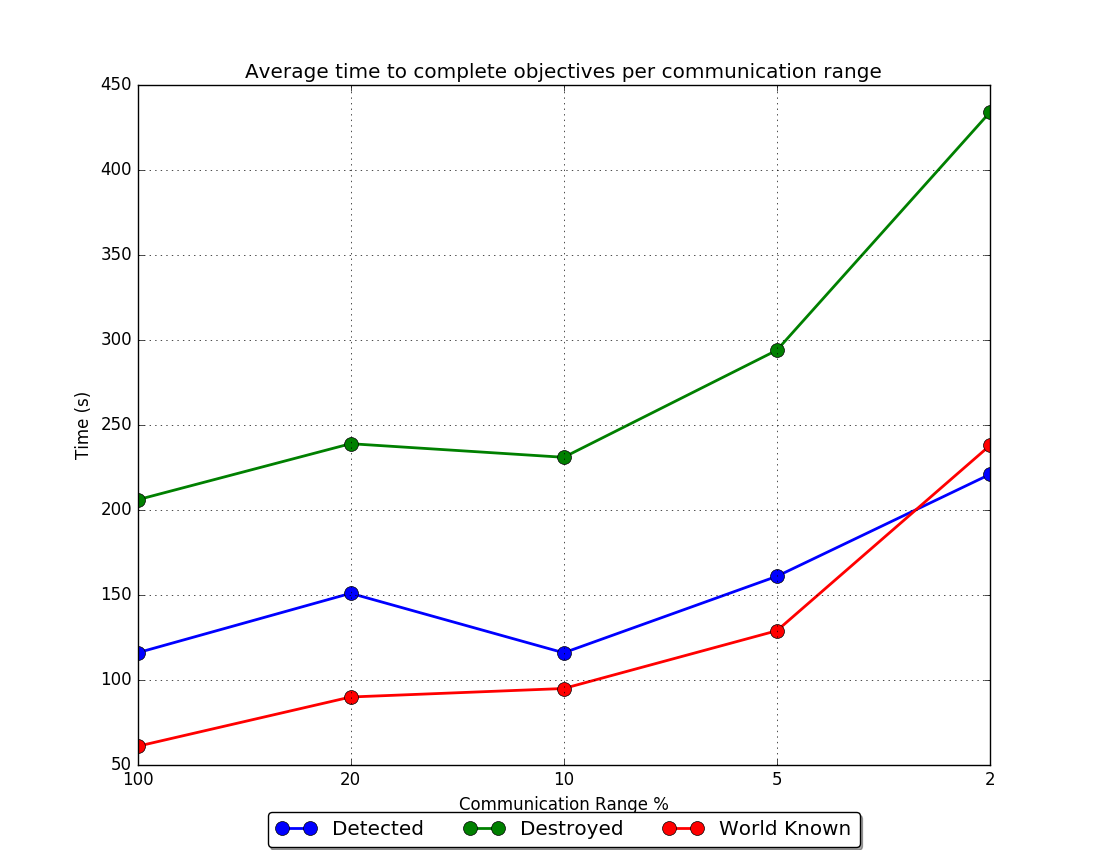
\includegraphics[width=\linewidth,height=4in,keepaspectratio=false]{averages.png}
%	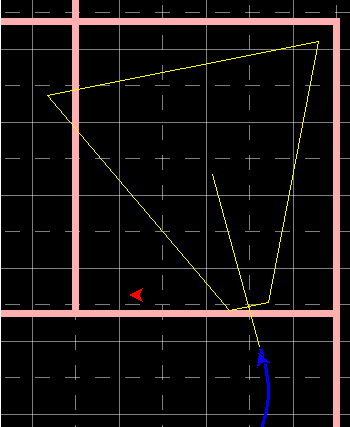
\includegraphics[scale=0.27]{wide_angle_scan.png}
	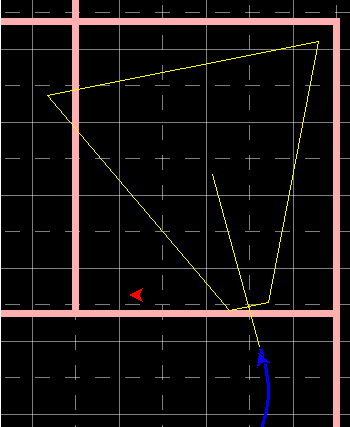
\includegraphics[width=\linewidth]{wide_angle_scan.png}
	\caption{A sensor performing a normal wide angle area scan.}
	\label{fig:wide_angle_scan}
\end{figure}

\begin{figure}[H]
	\centering
	%	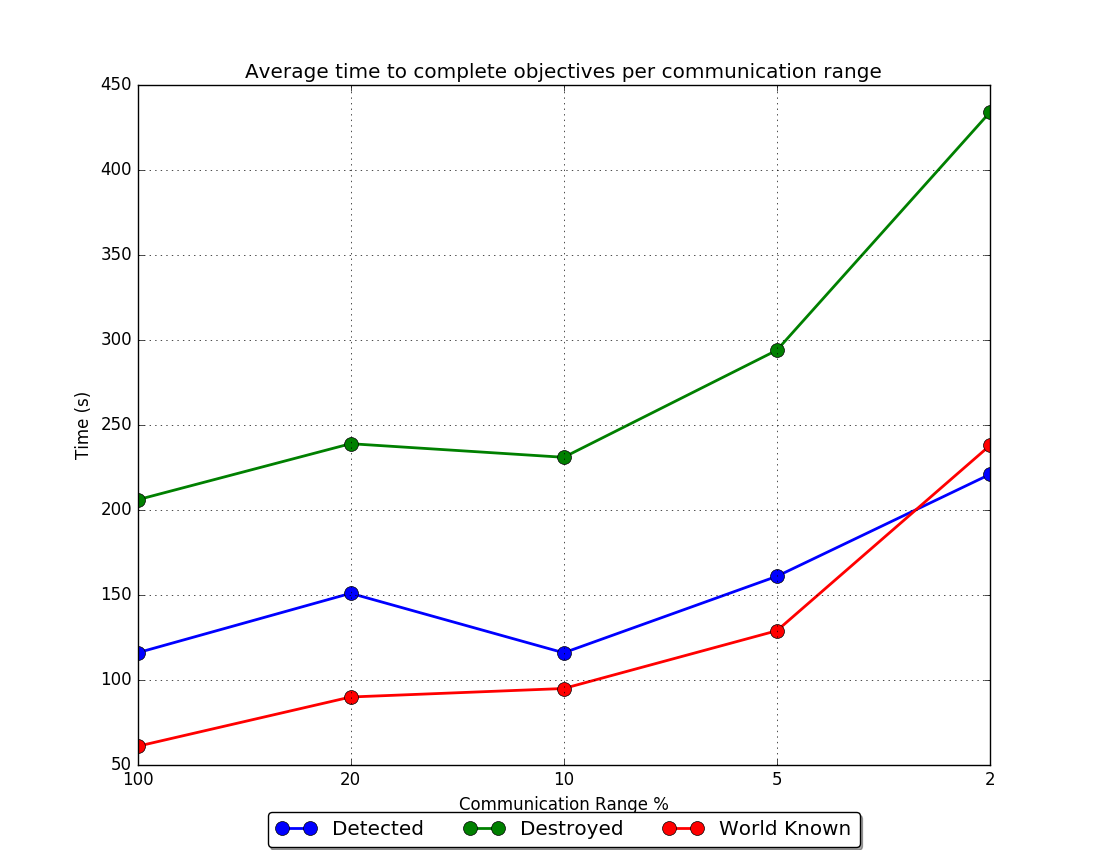
\includegraphics[width=\linewidth,height=4in,keepaspectratio=false]{averages.png}
	%	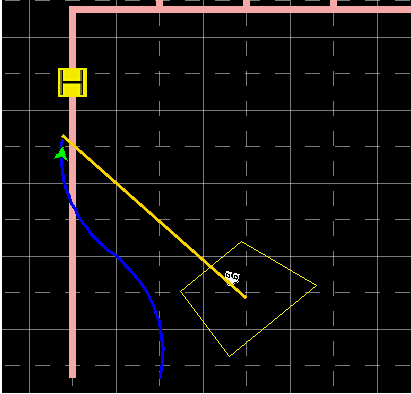
\includegraphics[scale=0.27]{narrow_scan.png}
	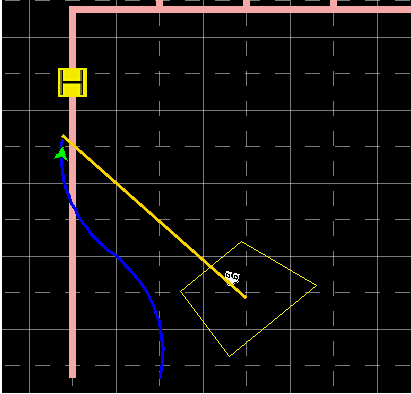
\includegraphics[width=\linewidth]{narrow_scan.png}
	\caption{A sensor performing a focused narrow scan of a destroyed target}
	\label{fig:narrow_scan}
\end{figure}

Similarly, each weapon type has a minimum and maximum launch range.  If a target is too close the weapon will not have enough time to properly acquire the target and fuse itself.  If a target is too far away the weapon's propulsion system will fall short of a lethal distance.  Weapons have limited steering capabilities so the host UAV must align its heading to the target within an acceptable launch angle region. A sample set of data characterizing weapons can be seen in table~\ref{tab:weaponType}.

% \todo{Do we care about a UAV being in the blast radius?}

\begin{table}[H]
	\caption{Weapon type definitions}
	\centering
	\rowcolors{1}{lightgray}{white}
	\label{tab:weaponType}
	\begin{tabular}{|p{1.4cm}|p{1.6cm}|p{1.2cm}|p{1.2cm}|}
		\hline
		Weapon Type & Launch Angle ($^{\circ}$) & Min Range (m) & Max Range (m)\\ \hline
		0 & 24 & 10 & 200 \\
		1 & 52 & 25 & 500 \\
		\hline
	\end{tabular}
\end{table}

%\section{Payload Probabilities}
\subsection{Payload Probabilities}
\label{sec:payload_probs}
This simulation uses realistic sensors in that they cannot perfectly detect targets or clear areas.  Each type of sensor has a probability of detecting if a target exists, a probability of confirming a target type, and an affinity for correctly estimating the heading of a target.  All of these attributes are user configurable and stored in a lookup table.  The values used for the experiment described in this paper are shown in table~\ref{tab:snsrTgtProb}.  These attributes are defined assuming perfect alignment with the target's \textit{Best Angle}.  Any variance from the target's \textit{Best Angle} will cause these probabilities and heading estimate to degrade.  For example, if a visible light spectrum camera is viewing a person's front we can see their face.  From this angle we can detect that we are looking at a person and confirm their identity.  If we orbit around behind the person we can still detect that a person is in front of the camera but the probability of confirming their identity correctly falls.

\begin{table}[H]
	\caption{Sensor to Target Probabilities}
	\centering
	\rowcolors{1}{lightgray}{white}
	\label{tab:snsrTgtProb}
	\begin{tabular}{|p{1cm}|p{1cm}|p{1cm}|p{1cm}|p{1cm}|}
		\hline
		Sensor Type & Target Type & Prob(Detect) & Prob(Confirm) & Heading Estimation Coefficient\\ \hline
		0 & 0 & 0.6 & 0.5 & 0.5 \\
		0 & 1 & 0.6 & 0.5 & 0.5 \\
		1 & 0 & 0.4 & 0.4 & 0.5 \\
		1 & 1 & 0.4 & 0.4 & 0.5 \\
		\hline
	\end{tabular}
\end{table}

Figure~\ref{fig:targetAngles} shows the gradient of performance scaling around a target based on the offset from the \textit{Best Angle}.  In this figure the target has a \textit{Best Angle} of $45^{\circ}$.  Any sensing or attacks at this angle will function with $100\%$ normal performance as defined in the probability lookup tables.  The direct opposite location at $225^{\circ}$ has a $0\%$ scaling value.  Any sensing or attack activities at this angle will not function at all.  Angles in between the \textit{Best Angle} and the opposite side will have their probabilities of success scaled by some percentage.

%\end{multicols}

\begin{figure}[H]
	\centering
	%	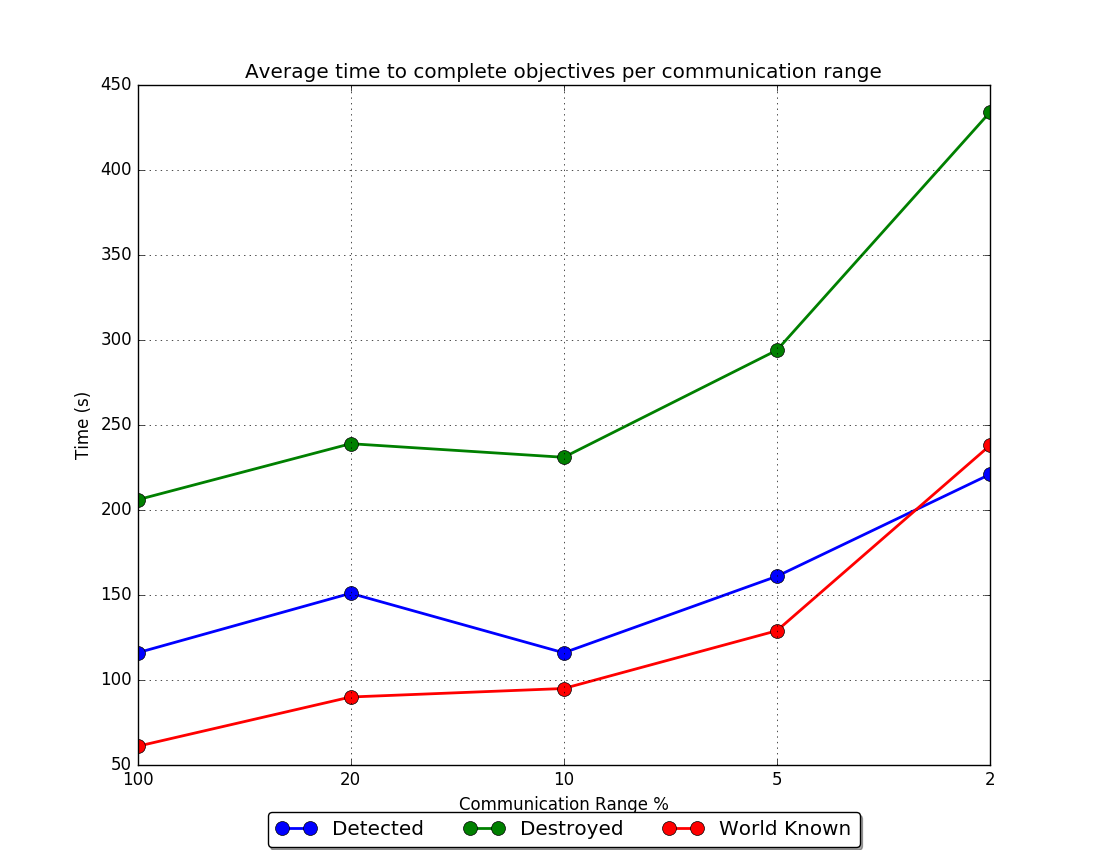
\includegraphics[width=\linewidth,height=4in,keepaspectratio=false]{averages.png}
	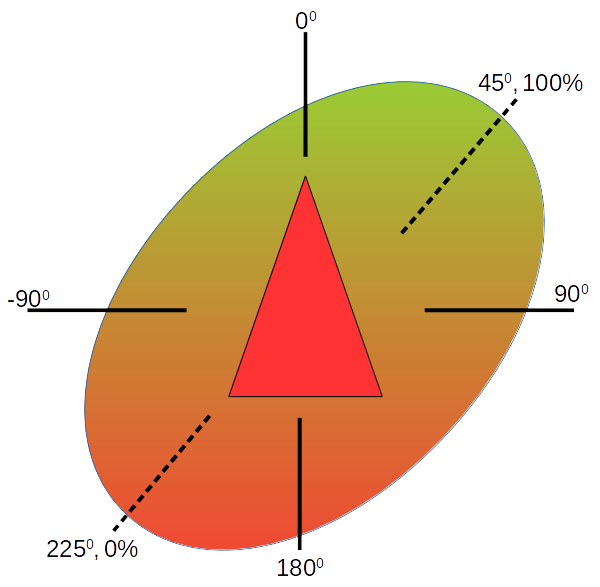
\includegraphics[scale=0.25]{targetAngles.png}
	\caption{Success scaling for a target with a best angle of $45^{\circ}$}
	\label{fig:targetAngles}
\end{figure}

Figure~\ref{fig:blue_red_angles} shows an example of two UAVs in blue interacting with a red target.  The relative angle between the target's heading and Blue 1's is close to the \textit{Best Angle} of $45^{\circ}$.  Blue 1 can sense or attack the target with little to no performance degradation.  The relative angle between the heading of the target and Blue 2 is much greater.  Therefore, Blue 2 will suffer a degradation in sensing and attack performance.

\begin{figure}[H]
	\centering
	%	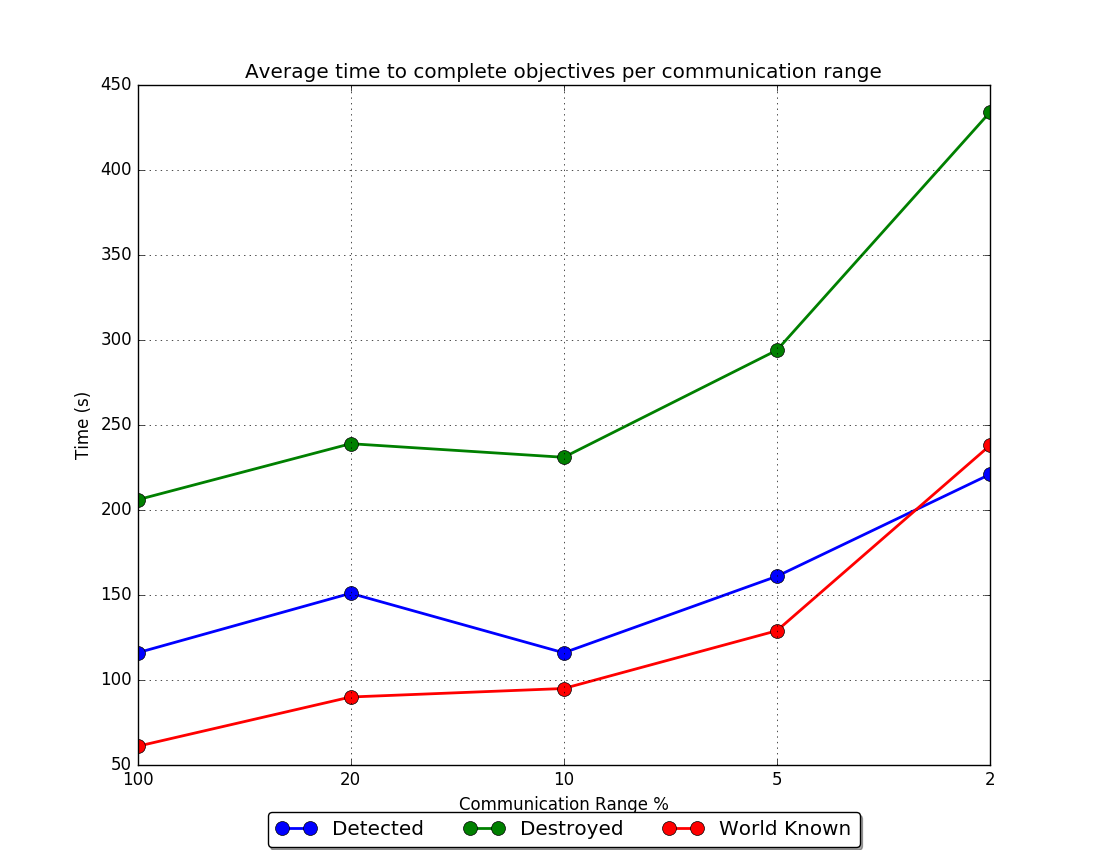
\includegraphics[width=\linewidth,height=4in,keepaspectratio=false]{averages.png}
	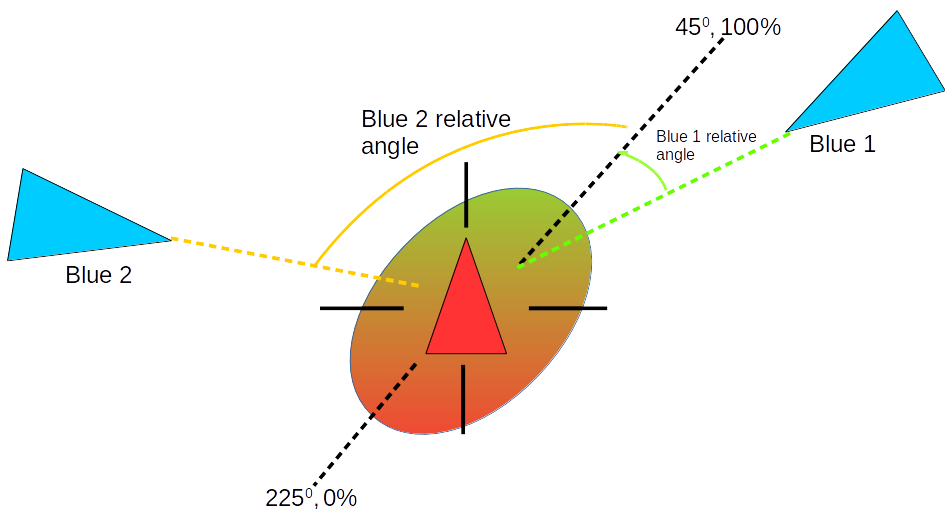
\includegraphics[scale=0.25]{blue_red_angles.png}
	\caption{Success scaling per relative angles}
	\label{fig:blue_red_angles}
\end{figure}

%\begin{multicols*}{2}

Weapons have a similar lookup table functionality in regards to the probability of successfully destroying a target assuming it is struck from its \textit{Best Angle}.  Any deviation from the \textit{Best Angle} causes a drop in the probability of destruction.  For example, let's imagine a car.  They have crumple zones to absorb impact energy to protect the occupants.  In a head-on collision the occupants are likely to survive because the front of the car will crumple and absorb a significant amount of energy.  If a car is struck along its sides in the door panels there is less protection for the occupants.  In this case the \textit{Best Angle} for a car is along the sides in the door panels. A sample set of data showing the probability of destruction mapping for each weapon and target combination in this experiment is shown in table~\ref{tab:wpnTgtProb}.

\begin{table}[H]
	\caption{Weapon to Target Probabilities}
	\centering
	\rowcolors{1}{lightgray}{white}
	\label{tab:wpnTgtProb}
	\begin{tabular}{|p{1.5cm}|p{1.5cm}|p{3cm}|}
		\hline
		Weapon Type & Target Type & Prob(Destruction)\\ \hline
		0 & 0 & 0.75 \\
		0 & 1 & 0.75 \\
		1 & 0 & 0.75 \\
		1 & 1 & 0.75 \\
		\hline
	\end{tabular}
\end{table}

%\textbf{TODO: chance of misclassification. Chance of empty cell detection}



\chapter{UAV Model}
Each UAV within the simulation is a self contained entity capable of acting and thinking on its own accord.  No UAV requires the presence of any other UAV or the aid of any external actor.  The swarm is made of multiple independent UAVs that share information and in doing so coordinate actions to complete the mission.  The simulation supports an arbitrary number of user defined UAV types (or platforms).

\todo{Mention each type has user defined payload}

\section{UAV Kinematics}
Each UAV type has a fixed speed and turning radius.  The fixed speed represents the aircraft's standard cruising speed that it will maintain throughout the simulation.  An example set of UAV type kinematic configuration data is shown in table~\ref{tab:uavKinematic}.

\begin{table}[h]
	\caption{UAV kinematic definitions}
	\centering
	\rowcolors{1}{lightgray}{white}
	\label{tab:uavKinematic}
	\begin{tabular}{|p{1cm}|p{2cm}|p{1cm}|}
		\hline
		UAV Type & Turning Radius (m) & Speed ($\frac{m}{s}$)\\ \hline
		0 & 300 & 30 \\
		1 & 150 & 50 \\
		\hline
	\end{tabular}
\end{table}

UAVs know their current 2D coordinate and heading.  This information is used to compute a path to any destination location and orientation.  In formal mathematics terms the kinematic model of a UAV is defined as \dots

\begin{align}
\dot{x} &= v \cos(\psi) \label{eq:uavChngX}\\
\dot{y} &= v \sin(\psi) \label{eq:uavChngY}\\
\dot{\psi} &= \{-constant, 0, constant\} \label{eq:uavTurnRate}\\
\dot{v} &= 0 \label{eq:uavAccel}\\
\psi_{constant} &= \frac{v*\sin(\pi)}{r} \label{eq:uavTurnRateDeriv}
\end{align}

\dots where $x$ and $y$ represent the UAV's current position on a Cartesian plane, $v$ is the UAV's fixed speed, $\psi$ is the UAV's heading, and $r$ is the UAV's turning radius.  Equations~\ref{eq:uavChngX} and \ref{eq:uavChngY} enforce that a UAV's position changes relative to its speed on a continuous trajectory.  Equation~\ref{eq:uavTurnRate} forces the UAVs to always turn at a known rate or not at all.  This allows for simplified trajectory planning using the equations for Dubin's Path described in section~\ref{sec:dubin}.  Equation~\ref{eq:uavAccel} states that the UAVs move at a constant speed.  The constant for the turn rate is computed as shown in equation~\ref{eq:uavTurnRateDeriv}.


\section{UAV Communications}
While each agent within the swarm is capable of self actualization mission performance improves when the agents work as a team.  To work as a team the UAVs must communicate with each other.  The simulation done in this work limits the communication range of UAV's to a percentage of the maximum world distance.  Given that the mission occurs in a square or rectangular environment the maximum world distance occurs between opposite corners along a diagonal that bisects the mission area.  By specifying the communication's range as a percentage of the world size the algorithms in this work are invariant of the physical world's size.

From a communications perspective the swarm can be thought of as a mobile ad hoc network (sometimes referred to as a MANET).  This is because the networking infrastructure between the UAVs is dynamic and unpredictable.  There are also no designated network control nodes.  Every UAV is equally likely to broadcast spontaneously.  A simple approach to make sure all agents within the swarm receive all communications is to 'flood` the broadcasts.  When an agent hears a particular message for the first time it is required to rebroadcast the message.  The advantage to this simple approach is that it requires no coordination or management overhead for communications support within the swarm.

While simple to implement this flooding approach has many drawbacks.  Many neighboring UAVs will likely have already heard the message themselves from the original source meaning there are redundant broadcasts.  Many neighboring UAVs will hear the message simultaneously and will jam each other when they all attempt to rebroadcast the message.  When the jamming occurs the data transmissions will be garbled if they succeed at all.  This is known as the broadcast storm problem as originally put forth by~\cite{bstorm}.

Finding ways to optimize MANETs and to eliminate the broadcast swarm problem is a whole field of research unto itself.  The research performed in~\cite{epidemicManets} and ~\cite{analysisOptNodeDen} are relevant to UAV swarms in that they find ways to minimize the number of needed transmissions and ways to reduce transmission power levels.  The standard approach is to not always rebroadcast a message when it is first heard and instead only rebroadcast based on chance.  This is known as the Probabilistic Flooding technique.  There are many variants to this technique with some described in~\cite{probFloodVariants}.  For our purposes the version described in~\cite{simpleProbFlood} was used.  In this case the the probability that a UAV will rebroadcast any individual message computed by equation~\ref{eq:probFlood} where $hop$ is the number of times the message has already been rebroadcasted and $num\_uavs$ is the number of UAVs in the swarm.  This equation states that when a message is first generated it is very likely it will be rebroadcasted but each subsequent broadcast becomes less likely to occur.

\begin{equation}
\label{eq:probFlood}
P(rebroadcast) = 1 - \frac{hop}{num\_uavs - 1}
\end{equation}

\section{UAV Tasks}
UAV's compete to selectively perform tasks in order to complete the mission.  The available tasks are \textit{Search}, \textit{Monitor}, and \textit{Attack}.  The Search task is always available for all UAVs to carry out.  The Monitor and Attack tasks are can only be executed in association with a suspected or confirmed target.\todo{Explain assignment states here?}

\subsection{Search}\todo{Uncertainty first used here but not defined}
No target locations within the simulated world are known \textit{a priori}.  The UAV's must discover all targets individually.  This was accomplished by mimicking the foraging behaviors of animals with an algorithm similar in principle to a \textit{L\'evy Flight}(\cite{humphries}) but adapted to a discrete world instead of a continuous world.  A search-and-track survey paper in~\cite{senanayake} highlights many other search algorithms to choose from.  The L\'evy Flight algorithm is a type of biased random walk.  The UAV foraging algorithm is enumerated in algorithm~\ref{alg:forage} in appendix~\ref{sec:algorithms}.  The algorithm will randomly select a grid cell within the world or it will divide the world into kernels, compute the uncertainty of each kernel, and randomly select a cell within the most uncertain kernel.  The kernel size must divide equally into the number of rows and columns in the world.

%https://en.wikipedia.org/wiki/L%C3%A9vy_flight

Once a search cell has been selected the UAV will fly towards it until another task takes precedence or the uncertainty in the cell falls below a user configured threshold.  The uncertainty in the cell changes when the UAV's sensors can reach it and when an update from another UAV in the swarm provides new data about the cell. If the uncertainty in the cell drops below the user configured threshold then the UAV will select a new cell to investigate.  Given that the UAV is within the most uncertain kernel when the selected cell becomes certain it will search another nearby cell.  Typically the UAV will search neighboring cells until the local kernel becomes more certain than other kernels in the world.  An atypical case occurs when the UAV selects a completely random location in the world.  The weighting between searching a kernel area versus random world locations is controlled by the $randomWeighting$ parameter in algorithm~\ref{alg:forage}.

While performing the search task UAV's point their sensor payloads towards the selected search cell even if they are not within range.  While traversing the world the UAV will opportunistically scan all cells encompassed by the sensor's field of view.


\subsection{Monitor}
The Monitor task requires a UAV to watch a potential target.  The UAV will point its sensing payloads at the target, confirm the target's identity, track the target, and perform a battle damage assessment after the target has been struck.  These steps are broken down into states within the Monitor task.  The monitor task state transitions are illustrated in figure~\ref{fig:monitor}. \todo{Need a page or section here?} 
\todo{Image formatting}

\begin{figure}[p]
	\centering
	%\includegraphics[width=\linewidth,height=\textheight]{imagefile}
	\includegraphics[scale=0.5]{uav_monitor_states.png}
%	\includegraphics{uav_monitor_states.png}
	\caption{Monitor sub-states}
	\label{fig:monitor}
\end{figure}

\subsubsection{En Route}
When a UAV first starts the Monitor task it begins flying towards the target and points its payloads in the target's direction.  As the UAV flies it continues to scan any cell within its payload's field of view until the target is within range.  Once the target is in sensor range the UAV transitions to the Target Confirmation state.  

When the UAV is in sensor range it will begin orbiting the target.  If the target moves more than some user configurable percentage of the sensor's range then the UAV will adjust it's flight path and recenter the orbit over the target's new location.

\subsubsection{Target Confirmation}
When the target is within sensor range the UAV will focus its sensors on the target.  This causes the sensors to stop performing a wide area scan and to zoom in on the target's suspected world cell location.  At this time the UAV is analyzing the sensor data to determine if the suspected target is a real target or if it's a false positive and no target exists.  No other targets can be detected in during this focused scan.  If the suspected target is fake then the UAV exits the Monitor task.  If the target is confirmed to be real then the UAV transitions to the Track Target state.  For purposes of this experiment the target confirmation analysis process was assumed to take 10 seconds.  No attempt was made to model real world physics of target identification from raw sensor data.

\subsubsection{Track Target}
In this state the UAV is continuing to point its payloads at the target but the sensors have resumed a wide area scan in hopes of finding other nearby targets.  The UAV stays in this state until the target outruns the UAV's sensors and is lost or the target is struck by a weapon.  When the UAV first enters this state it requests a weapon's strike on the target from the swarm.  The details of the weapon's strike request are presented in section~\ref{sec:uavBelief}.

\subsubsection{Battle Damage Assessment}
When the monitoring UAV detects a weapon's strike on the target it will transition from wide area scan tracking to narrow focused scans of the target's location.  As in the Target Confirmation state during this focused scan no other targets can be detected and the certainty of other cells do not change.  This state represents the time it takes for the UAV to analyze its sensor data to determine if the target was destroyed or if it is still active.  Again, for purposes of the experiment it was assumed that battle damage assessment (BDA) takes 10 seconds to complete.  No attempt was made to model real world physics of target status from raw sensor data.

If the target is still active after the weapon's strike the UAV will transition back to the Track Target state and request another strike from the swarm.  If the target was destroyed then the UAV will exit the Monitor task.


\subsection{Attack}
The Attack task mechanics are similar to the Monitor task in that the UAV will fly towards the target and point all of its sensors at the target.  The UAV will plot a course such that its heading is aligned with the best attack angle relative to the heading of the target.  The UAV will re-plot a new course if the target moves a significant distance.  This distance is user configurable.  The UAV will wait until the distance to the target is below some percentage of the weapon's max range before firing.  For purposes of this experiment the percentage was set to 80\%.

The weapon time-of-flight is not modeled.  Weapon strikes are considered instantaneous.  When the weapon is deployed the UAV has completed the task.  The UAV may assign itself a new task and begin maneuvering to a new destination.  However, the UAV performing the Monitor task may request another weapon strike from the swarm if the target was not destroyed.  Therefore the UAV that completed the Attack task might decide to perform it again since it's likely the closest strike platform available.  The details of this process are explained in section~\ref{XXXX}.\todo{Fix reference.} 




\section{Uncoordinated Tasking}
\label{sec:uncoordTasking}
\todo{Lots of references to contract network and auction papers}

Task allocation is accomplished using a decentralized process in the swarm.  Previous work in distributed or decentralized task allocation has been done in . Due to the desire for real world applicability of the algorithms presented here complex evaluation or large data packets were shunned. It is inspired


\subsection{Monitoring a Target}

\subsection{Attacking a Target}

Flow charts
\begin{figure}[h]
	\centering
	%\includegraphics[width=\linewidth,height=\textheight]{imagefile}
	\includegraphics[scale=0.5]{uav_activity_attack.png}
	\caption{UAV Attack Activity}
	\label{fig:uavAttackActivity}
\end{figure}



Starvation of search task

limited comms range

\begin{table}[h]
	\caption{UAV sensor payload configuration}
	\centering
	\rowcolors{1}{lightgray}{white}
	\label{tab:uavSensorMap}
	\begin{tabular}{|p{1cm}|p{1cm}|p{1cm}|}
		\hline
		UAV Type & Sensor Type\\ \hline
		0 & 1 \\
		1 & 0 \\
		\hline
	\end{tabular}
\end{table}


\todo{Insert sim data for weapon numbers}
\begin{table}[h]
	\caption{UAV weapon payload configuration}
	\centering
	\rowcolors{1}{lightgray}{white}
	\label{tab:uavWpnMap}
	\begin{tabular}{|p{1cm}|p{1.5cm}|p{2cm}|}
		\hline
		UAV Type & Weapon Type & Initial Quantity\\ \hline
		0 & 0 & 2 \\
		0 & 1 & 2 \\
		1 & 0 & 5 \\
		1 & 1 & 5 \\
		\hline
	\end{tabular}
\end{table}

\chapter{Belief Model}
\label{sec:uavBelief}
The belief model is the fundamental piece that allows the swarm to function as a cohesive group instead of many individuals in the same local area.  The belief model consists of data about all cells in the world grid and data about all known targets.  Each UAV has its own unique belief about the current state of the world.  Periodically the UAVs broadcast their belief to everyone nearby within communications range.  When a UAV receives another UAV's belief model the receiver merges the incoming data into their own internal belief model.  By this mechanism data is shared and propagated throughout the swarm.  Therefore the communication range of each UAV is a limiting factor in the effectiveness of the swarm.  Like all team based exercises effective communication is critical to success.\todo{Add graphic of comm ranges}  

\section{Cell Beliefs}\todo{Image of cell attributes}
Prior to beginning the mission the geographic area is tessellated into a rectangular grid of $M$ rows and $N$ columns.  The actual physical size of the cells is irrelevant to the algorithm.  However, scanning half a cell and declaring it empty while a target sits in the other half is erroneous.  Therefore a constraint exists such that the grid cells must be small enough so that the smallest field-of-view of all the sensors must be able to completely encompass a grid cell in a single sensor frame.  This constraint prevents the noted error condition.

Each cell in the world grid is identified by a row and column index.  Each cell contains a probability of being empty ($P(empty)$) and a timestamp of when this data was last updated.  This is commonly called a Grid Based Occupancy Map. The probability value is updated in a Bayesian fashion by sensor scans \todo{Explain this process}during each time step of the simulation similar to~\cite{waharte}.  This probability is then used to derive a Discrete Shannon Uncertainty (also known as Shannon Entropy~\cite{shannon}) value.  A Shannon Uncertainty curve is zero when $P(empty)$ is 0\% or 100\% since in those edges cases we know for certain if the cell is empty or not.  Conversely a Shannon Uncertainty curve is at its peak when we know nothing for certain when $P(empty)$ is 50\%.  Nominally a Shannon Uncertainty curve varies from zero to roughly 0.301 (when $P(empty) = 0.5$).  The equation can be see in~\ref{eq:shannon}.  For ease of use it can be scaled from zero to one by dividing~\ref{eq:shannon} by it's maximum value of $U_{max}$ shown in~\ref{eq:shannon_max}.  The results of this are plotted in figure~\ref{fig:shannon}.

\begin{equation}
	\label{eq:shannon}
	\begin{split}
		U = & -P(empty) * \log_{10}(P(empty)) \\
            & - ( 1-P(empty) * \log_{10}(1-P(empty)))
	\end{split}
\end{equation}

\begin{equation}
	\label{eq:shannon_max}
	\begin{split}
		U_{max} = & -0.5 * \log_{10}(0.5) \\
		          & - (0.5 * \log_{10}(0.5)) \\
		          & \approx 0.301
	\end{split}
\end{equation}

\begin{figure}[h]
	\centering
	%\includegraphics[width=\linewidth,height=\textheight]{imagefile}
	\includegraphics[scale=0.4]{shannon.png}
	\caption{Shannon Uncertainty}
	\label{fig:shannon}
\end{figure}

The goal of the mission is to destroy all the unknown targets in the search-and-destroy scenario.  Therefore the desired end state of the UAVs' shared belief model is to reduce the Shannon Uncertainty of each world cell to 0\%.  In this case all targets have been destroyed and all locations in the world have been explored.  In practice the world cells are never all driven to 0\% at once.  There is a global certainty decay rate that is applied to the cell beliefs at every time step.  It slowly drives $P(empty)$ back to 50\% over time.  This models the fact that unless a UAV is watching a cell they cannot know with 100\% certainty what is going on within that cell.  There is a chance that a moving target that has somehow evaded detection could be occupying a previously scanned world cell location.  So instead of requiring the uncertainty of all world cells to be at 0\% to end the mission we only require that all cells be driven below a user defined threshold percentage.

\section{Target Beliefs}
When a UAV detects something that might be a target it adds a Target Belief to its Belief Model.  The Target Belief contains an estimation of the target's location and orientation.  It also contains a list of all possible target types and an associated probability that the detected target is the corresponding type of target. The list of target type probabilities within a Target Belief always sum up to one.  At initialization all target types are equally likely.  As time progresses and more sensor scans of the target are completed the probabilities per target type will converge to a single type.  This is accomplished with the Bayesian update model described in XXX.\todo{Explain sensor bayesian process}  

In addition to estimated data about the actual target Target Beliefs encapsulate information about the tasks performed on the target.  This tasking data is called a Target Task Status object\todo{Need better word or name}.  This data is used for coordinating activities within the swarm.  Since the swarm of UAVs has no centralized control system to allocate task assignments this process must be done by mutual consent within the swarm.  Each Target Belief has a Target Task Status that denotes who is performing tasks on a target and if the task is still eligible for others to take over.  The Target Task Status includes the following attributes.

\begin{description}
	\item [Monitor UAV ID] The ID of the UAV who has the best monitor score.
	\item [Monitor UAV Score] The best known score for monitoring the target.
	\item [Monitor Task State] An enumeration describing the current phase of task coordination for monitoring.
	\item [Monitor Update Timestamp] The time when the monitor data was last updated.
	\item [Attack UAV ID] The ID of the UAV who has the best attack score.
	\item [Attack UAV Score] The best known score for attacking the target.
	\item [Attack Task State] An enumeration describing the current phase of task coordination for the attack.
	\item [Attack Update Timestamp] The time when the attack data was last updated.
	\item [Target Destroyed Flag] A flag indicating if the target has been destroyed or not.
\end{description}

The Task State enumerations control when and who may bid on tasks.  There are subtle differences in their uses between the monitor tasks and the attack tasks.  These are explained in detail in  section~\ref{sec:uncoordTasking}.


\begin{description}
	\item [NO TASK] This is the initial null condition given to the monitor and attack tasks.  In the monitor case it means the target was just discovered and no one has had a chance to process it.  In the attack case it means no one has confirmed that the target should be destroyed.
	\item [Open] The task is open to any and all bids.  No one has attempted to claim the task yet.
	\item [Enroute] This means the UAV with the corresponding ID is on its way to the target to perform the corresponding task.  Anyone else could overrule if they have better score than current best UAV.
	\item [Performing] The UAV with the corresponding ID is now performing the action.  No one else may overrule or otherwise subsume the action regardless of their score.
	\item [Complete] The task has been completed by the UAV with the corresponding ID.  In the monitor case the target has been confirmed as destroyed.  In the attack case a weapon has been deployed but the target is not necessarily destroyed.
\end{description}

\section{Merging Beliefs}
Each UAV in the swarm periodically broadcasts its internal Belief Model.  The entire model is encoded and transmitted to all other swarm members within communications range.  When a UAV receives another swarm member's belief model it must be merged with the receiver's internal belief.  No UAV completely trusts any other UAV in the swarm.  All data is merged in a weighted or filtered fashion.  No data is copied 100\% as-is since there are no guarantees that any one UAV is perfectly correct about anything.  The mering process in this work is an implementation of the Fusion Update technique described in~\cite{shem} for merging multiple values of uncertainty.

Merging Cell Beliefs is a simple process.  The formal algorithm can be found in~\ref{alg:mergeCell}\todo{Future work: Sensor type expertise should weigh into this}.  In short the receiving UAV compares every single world cell with its counterpart in the sending UAV's data.  If the last update timestamp of the incoming cell data is more recent than the currently stored data then the cell data is merged.  The merge process is a weighted average.  When the merge occurs the receiving UAV's timestamp is set to the timestamp of sending UAV's data.  This prevents future belief broadcasts from the same sending UAV to trigger another re-merging of the exact same cell data.  This also prevents the same data from re-merging if a third party UAV forwards the belief data. 

Table~\ref{tab:exampleCellMerge} shows an example of merging a single cell.  At some time in the simulation UAV 1 believes cell $[2, 6]$ has a 20\% of being empty (or in other words an 80\% chance that something is there). This probability was last updated at time 1234.  UAV 1 has broadcasted this belief data and UAV 2 has received it.  UAV 2 believes there is a 50\% chance that the same cell is empty but this data was last updated a long time ago at time 22.  Therefore UAV 2 will merge UAV 1's data for this cell.  Since alpha is set to 0.6 the new $P_{2,6}(empty)$ for UAV 2 is $0.6*(0.2) + (1-0.6)*(0.5)=0.32$.  After the merging is complete UAV 2's $P(empty)$ value is set to $0.32$ and the last update timestamp is set to UAV 1's timestamp.

\begin{table}[h]
	\caption{Example cell merging with $alpha=0.6$}
	\centering
	\rowcolors{1}{lightgray}{white}
	\label{tab:exampleCellMerge}
	\begin{tabular}{|r|c|c||c|c|}
		\hline
		                & \multicolumn{2}{c||}{Before Merge} & \multicolumn{2}{c|}{After Merge} \\
		\hline
		UAV             & 1   & 2                            & 1   & 2 \\
		\hline
		$P_{2,6}(empty)$& 0.2 & 0.5                          & 0.2 & 0.32 \\
		\hline
		Timestamp       & 1234& 22                           & 1234& 1234 \\
		\hline
	\end{tabular}
\end{table}

Merging Target Beliefs is more complicated but uses a similar weighted averaging technique as merging Cell Beliefs.  The model in this paper assumes that the UAV's are able to perform target track fusion (also known has cross-track correlation) amongst themselves and assign each track a unique ID such as in~\cite{stroupe}, \cite{barooah}, and~\cite{spillings}.  This process is outside the scope of this paper.

As stated earlier Target Beliefs have an estimated location, orientation, and list of target type probabilities.  Now we assume they also have a unique identifier assigned by the target track fusion process.  This unique identifier is used as a first pass comparison filter when merging Target Belief data.  If the receiving UAV does not have any data for the incoming Target Belief it simply copies it verbatim.  If the receiving UAV already has data for the Target Belief then a more detailed inspection is required.  Target Beliefs only get merged if the received data is newer than the currently stored data.  In this case the estimated target orientation, position, and list of type probabilities are all averaged with a user defined weighting against the incoming data.  The formal algorithm is defined in algorithm~\ref{alg:mergeTarget}.

The Target Task Status within a Target Belief is also merged with incoming data.  Instead of performing weighted averages logic must be applied to determine if the task status data is still live and active or if the data is transmitted for historical reference only.  The formal algorithm is defined in algorithm~\ref{alg:mergeTaskStatus}.

\chapter{Task Allocation}
\label{sec:uncoordTasking}

Assigning tasks amongst a group of workers is a well known problem with many facets and variants.  In our case we have a group of UAVs flying around with different capabilities.  The UAVs coordinate and cooperate but there is no centralized controller or manager.   In theory having a centralized controller with perfect information could produce the most optimal configuration of task allocations for the entire swarm.  In practice achieving such a system is difficult since it requires a large amount of communication and introduces a single point of failure.  Algorithms that create an optimal solution given perfect information can take a long time to run.  So even if we have a suitable communications network the responsiveness of the centralized controller introduces another potential problem especially as the size of the swarm or number of potential tasks increases.

Fully decentralized controllers cannot guarantee perfectly optimal task allocations but they can usually provide ``good enough'' allocations.  An example of this is proven in~\cite{auction_linear_approx} where the distributed algorithm came within a linear approximation of the perfect global optimum solution.  Decentralized controllers use imperfect local knowledge and can operate very fast in comparison to centralized controllers due to their inherent parallelism.  Decentralized controllers also offer failure redundancy and reductions in performance requirements of the communications network.  It's possible a communication network may not be needed at all as with stigmergic systems.

Two common approaches to distributed task allocation are market based algorithms and behavioral algorithms.  On the spectrum from fully centralized to fully decentralized these algorithms lie somewhere in the middle in order to capitalize on the strengths of both approaches.

\section{Market based allocation}

The Auction Algorithm borrows concepts from economics to model an auction as its name implies.  A centralized version was proposed in in~\cite{auction_derive} and enhanced in later revisions by the same author.  The author created a distributed version of the Auction Algorithm in~\cite{auction_parallel}.  The algorithm requires an agent to start an auction for some task to be completed.  Typically the agent that first detects a task that needs to be complete starts the auction.  The agent broadcasts out a message with details about the task to the swarm.  Other agents then formulate a bid for the task and send their responses back to the auctioning agent.  The auctioneer waits for the bid responses and analyzes them.  The auctioneer could declare a winner or it could rebroadcasts the current best bid and wait again for further responses with higher bids.  

This is a generic description of the Auction Algorithm.  There are many variants and derivatives that change how bids are generated, how the auction is closed, and how to handle communication failures.  There are even variants to allow multiple agents to perform a task together as a team in~\cite{auction_team}.  The core feature of the algorithm is the temporary centralized auctioneer per newly discovered task.  For this to work the auctioneer must to be able to communicate with local agents and be able to compare their bid responses.  It also requires each agent to understand what it takes to accomplish every possible task.

Another market based system is the Contract Net protocol first introduced in~\cite{contract_net}.  It could be considered a specialization or superset of the Auction Algorithm.  This protocol breaks a task into subtasks and allows each subtask to be auctioned independently. It defines a meta-language within the allocation process for describing tasks and the resources required to complete them.  It provides mechanisms for reporting on the status of tasks and returning information once a task in complete.  This allows more cooperation between agents and a potential for better global optimization since each sub-task can be performed by the best agent available instead of a single agent performing all subtasks within a task.  The trade-off for this better global optimum performance is a requirement for more communication to handle the subtask allocation and coordination.  As with the Auction Algorithm many variants of the Contract Net protocol have been created as described in~\cite{contract_survey} and ~\cite{contract_equity}.

\section{Behavior based allocation}

Behavior based algorithms are algorithmic representations of phenomenon seen in humans and animals. They differ from the market based solutions in that agents ``take'' or ``volunteer'' for a task instead of being ``assigned'' a task.  For example in~\cite{ant_colony_opt} a team of robots cooperated in a fully decentralized fashion and used the Ant Colony Optimization(~\cite{wiki:aco}) algorithm for task allocation.  All of the robots were identical in form and function.  Tasks could require one or more robots.  Each robot used its own sensors to create a model of the environment and to generate a list of tasks to be accomplished.  A robot would then move about and observe a task.  It would then determine if enough robots were simultaneously working on a task together.  If not then it would join in the effort otherwise it continued onto another task in the environment.  In this case no active communication occurred and tasks were passively taken.

Stigmergy is another common behavior based system.  In stigmergic systems data is not directly passed from one agent to the next.  Instead the environment is modified by the agents and in doing so data is encoded.  Other agents who then observe the modified environment will learn about the data left behind from the previous agent.  In~\cite{stigmergy_building} a swarm of agents moved 2D blocks around to create a 2D structure.  No direct communication between the agents occurred.  Instead the agents were all programmed with rules indicating if they did not have a block that they should find one and if they have a block then they should find another collection of blocks that match some known pattern in their memory.  Once they found a pattern they dropped the block they were carrying to extend the collection or pattern.  In this fashion jumbled piles of blocks were turned into 2D structures.  In this case no active communication occurred and tasks were passively taken.

Another common example of behavior based task allocation are pheromone systems.  In these systems agents of the swarm deposit a physical or virtual pheromone at a location.  The type of pheromone deposited indicates the type of task that can be performed at the location.  Over time these pheromones decay and disappear or seep into nearby locations.  The seepage of pheromones into nearby locations helps agents find and perform tasks by following the gradient of the pheromone's strength.  As with the other task allocation algorithms there are many variants and techniques for handling the details of the pheromone system.  In~\cite{pheromone} an ant colony was modeled in that the agents left the nest and foraged for food.  As the agents explored they left behind a ``to nest'' pheromone.  This pheromone helped guide the ant agents back to the nest.  When the ant agents found a source of food they would deposit a ``to food'' pheromone.  When the food carrying agents made it back to the nest by following the ``to nest'' gradient other ants would notice the newly deposited ``to food'' pheromone.  The other agents would then follow the ``to food'' pheromone to the food source and return to the nest therefore restrengthening the ``to food'' pheromone creating a positive feedback loop.  A pheromone system like this can obviously be modeled with literal real chemical pheromones left behind by robotic agents.  It can also be modeled virtually by agents broadcasting a pheromone strength number in their belief models that are communicated with the rest of the swarm.  In this case active communication is used but tasks are passively taken instead of being assigned.\todo{Discuss TRA.pdf? Motivational behaviors?}

\section{WORKING TITLE: My Allocator}\todo{Needs a name}

The allocation scheme used in this work is more closely aligned to the fully decentralized end of the spectrum.  If other agents exist within communications range they will share their belief models but they will not otherwise directly engage each other.  Periodically agents analyze their belief model to find the best action they can do.  There are only two strongly enforced rules to control who performs a particular task.  

\begin{enumerate}
	\item The agent with the best Monitor or Attack score in the Target Belief data structure gets to perform the task.
	\item Once an Attack task's state is set to \textit{Performing} no other agent may claim the task regardless of rule 1.
\end{enumerate}

Rule 1 states that a ``survival of the fittest'' situation occurs.  If multiple UAVs compete for the same task then the strongest agent wins the task.  Scores are computed based on the UAV's ability to perform the task and their current distance from the task.  While it is theoretically possible for ties in scoring to occur in practice it is inconsequential.  The ability to perform a task has many variables and distances to the targets are always changing.  Each UAV's score will change slightly at the next periodic update which occurs multiple times a second.

When a task's state changes to \textit{NO TASK}, \textit{Open}, or \textit{Enroute} any UAV may attempt to claim it.  Claiming occurs when an agent is close enough to begin performing the action and they set the Task State to \textit{Performing}.  An agent may choose to stop performing a task by resetting the task's state to \textit{Open}.  When an agent claims an attack task rule 2 comes into affect and no other UAV may take the task.  UAVs performing the Monitor task may be overridden if another UAV comes within range with a significantly better score.  The definition of significantly better is definable by the operator as a percentage.   This helps to prevent churn in the monitoring process but allows a much better sensor to be utilized if it presents itself.  Either way, someone is always watching the target.\todo{write out algorithm for task claiming}

These rules only work in an environment where no agent lies.  An agent can have out of date information and faulty sensors but they cannot actively lie.  All information is timestamped using a synchronized clock so stale data is a recoverable error and accounted for in all comparison and merging processes.  Faulty sensors can be overcome by other members of the swarm repeatedly contradicting the bad data.

Tasks start in the \textit{NO TASK} state when they are first discovered.  The discovering agent will add the task to their belief model and broadcast it out locally.  Other agents may hear about the new task and rebroadcast it out again when they next transmit their belief model.  In this fashion the task will propagate through the network.  However, there is a latency in the logic processing between agents near the task and those farther away.  It takes time for the task to hop from the interior to the exterior of the swarm.  During this timespan agents closer to the task may already begin to posture to claim it while those farther away are just first hearing about it.  There is a weighting factor set by the operator to specify if they prefer the closest UAV to perform the task or if they prefer the best equipped UAV to perform the task.  This weighting factor allows UAVs far away from the initial task announcement a chance to claim the task.

When a UAV thinks it can claim a task it sets the Target Belief data with the computed score, the UAV's ID, and sets the Task State to Enroute.  Other UAVs will hear these updates at the next periodic belief model broadcast.  Simultaneously other UAVs could believe they will claim the task as well and eventually multiple UAVs could arrive near the task.  While they are all enroute their beliefs propagate through the network and merge with others.  Eventually some of the UAVs will hear that they are not the best suited for the task and will go find some other task to perform.  This competition period emulates the centralized controller strength in that someone coordinates who gets to perform the task.  In this case the centralized controller changes swiftly based on who the dominant UAV is at the time.  The dominant UAV effectively guards their territory like an animal until a stronger one appears.

This simple ``survival of the fittest'' mechanism has many benefits.  There is very little communication required.  UAVs share their belief model of the world which is just a static data dump with well defined merging procedures.  Other UAVs hear this whole data packet or they hear nothing at all.  There is no need to maintain and manage temporary communication channels to facilitate negotiations or transactions like in market based algorithms.  This mechanism is most closely related to pheromone models with the addition that agents know who laid down the pheromone.  Each UAV has their own unique pheromone signature.  This means the control laws for guiding the aircraft consolidate down to a series of strength comparisons with no higher level logic.


 in . Due to the desire for real world applicability of the algorithms presented here complex evaluation or large data packets were shunned. It is inspired
%\chapter{Performance Metrics}
Lorem ipsum dolor sit amet, consectetur adipiscing elit, sed do eiusmod tempor incididunt ut labore et dolore magna aliqua. Ut enim ad minim veniam, quis nostrud exercitation ullamco laboris nisi ut aliquip ex ea commodo consequat. Duis aute irure dolor in reprehenderit in voluptate velit esse cillum dolore eu fugiat nulla pariatur. Excepteur sint occaecat cupidatat non proident, sunt in culpa qui officia deserunt mollit anim id est laborum.
\chapter{Discussion of Results}
\label{chap:results}

\section{Performance Metrics}
The \textbf{TODO: INSERT MODEL NAME} model was implemented and simulated in a custom computer program.  The model's performance was measured in three ways; time to detect all targets, time to destroy all targets, and the time it took to ``know'' the whole world.  Using these metrics conclusions can be drawn about the model's capabilities.

\begin{description}
	\item [Time to detect all targets] The amount of time from the start of the simulation until all targets in the simulation have been detected by any UAV at least once.  This is implemented by using target truth data and maintaining a corresponding status flag per target that is set once the target is detected.  Once all of the flags have been set then all targets have been detected at least once.  When this evet occurs the time is recorded.
	
	\item[Time to destroy all targets] The amount of time from the start of the simulation until all targets have been destroyed.  This is implemented by using target truth data and recording the time when all targets have been destroyed.
	
	\item[All world known] This is the amount of time from the start of simulation until over half of the UAVs in the swarm reduce the average uncertainty of all of their Cell Beliefs below a user defined threshold.
\end{description}


\section{Experiment Configuration}
For this experiment 10 random worlds were generated each with 2 mobile targets, 4 static targets, and 5 UAVs.  The simulated worlds were configured as a 2.5 by 2.5$km$ area subdivided into 15 rows and columns.  A rendering of each generated world is included in section~\ref{sec:world_images}.

The mobile targets moved at $10m/s$ and were best hit from $\pm115^{\circ}$ from their front.  Static targets were best hit from $\pm45^{\circ}$.

Two types of UAVs were modeled.  One is a fast long range ISR platform and the other is a slow strike platform.  The ISR platform is type 0 in table~\ref{tab:uavKinematic}.  The strike platform is type 1 in table~\ref{tab:uavKinematic}.  The ISR platform carries sensor 0 defined in table~\ref{tab:sensorType} and has no weapons.  The strike platform has sensor type 1 defined in table~\ref{tab:sensorType}.  The strike platform carries 4 rounds each of weapon types 0 and 1 defined in table~\ref{tab:weaponType}.  Ideally this is more than enough munitions to complete the missions even with a significant amount of misses.  The performance of these sensors and weapons against the targets are defined in tables~\ref{tab:snsrTgtProb}, ~\ref{tab:snsrTgtMisClassProb}, and \ref{tab:wpnTgtProb}.  Static targets are target type 0 and mobile targets are type 1.  The sensors all have a $10\%$ chance of misclassifying any target type as the other type as listed in ~\ref{tab:snsrTgtMisClassProb}.

The threshold for the ``all world known'' metric was set at 0.3. To obtain a Shannon Uncertainty of 0.3 or lower requires having a $P(empty) < 5\%$ or $P(empty) > 95\%$.

\section{General Results}

The simulation was ran for all 10 worlds with the same random seed.  This process was repeated 5 times in order to measure the effects on mission performance with a varying communication range.  The results of these simulation runs were averaged together and are shown in table~\ref{tab:avgResults} and plotted in figure~\ref{fig:averages}.  Standard deviations are supplied in table~\ref{tab:stdDevResults}.  The complete raw time data per world and per communication range can be found in section~\ref{sec:raw_data}.  The standard deviations are \textbf{TODO: Box plots} \texbf{TODO: explain goals}

\begin{table}[H]
	\caption{Average time to complete objectives}
	\centering
	\rowcolors{1}{lightgray}{white}
	\label{tab:avgResults}
	\begin{tabular}{|p{1.25cm}|p{1.5cm}|p{1.75cm}|p{1.5cm}|}
		\hline
		Comm. Range \% & Average time all detected (s) & Average time all destroyed (s) & Average time world known (s)\\
		\hline
		100 & 116 & 206 & 61  \\ \hline
		20  & 151 & 239 & 90  \\ \hline
		10  & 116 & 231 & 95  \\ \hline
		5   & 238 & 279 & 242 \\ \hline
		2   & 380 & 554 & 339 \\ \hline
	\end{tabular}
\end{table}

\begin{table}[H]
	\caption{Standard deviation to complete objectives}
	\centering
	\rowcolors{1}{lightgray}{white}
	\label{tab:stdDevResults}
	\begin{tabular}{|p{1.25cm}|p{1.5cm}|p{1.75cm}|p{1.5cm}|}
		\hline
		Comm. Range \% & Std. Dev. for time all detected (s) & Std. Dev. for time all destroyed (s) & Std. Dev. for time world known (s)\\
		\hline
		100 & 52 & 58  & 29  \\ \hline
		20  & 62 & 53  & 68  \\ \hline
		10  & 53 & 77  & 48  \\ \hline
		5   & 93 & 85  & 50  \\ \hline
		2   & 90 & 105 & 112 \\ \hline
	\end{tabular}
\end{table}



The $100\%$ communication range case serves as a comparative baseline against a perfect global communication network.  In this case all UAVs are able to communicate with all other UAVs at all times.  As expected a perfect global and centralized communication network always performs better than a network with limited ranges.  The interesting point of comparison is that the $10\%$ and $20\%$ range cases come very close or match the $100\%$ case in performance.  This can be seen in figure~\ref{fig:averages} and in the ratios listed in table~\ref{tab:avgResultsRatio}.

\begin{table}[H]
	\caption{Ratio of time to complete objectives compared to 100\% range}
	\centering
	\rowcolors{1}{lightgray}{white}
	\label{tab:avgResultsRatio}
	\begin{tabular}{|p{1.25cm}|p{1.5cm}|p{1.75cm}|p{1.5cm}|}
		\hline
		Comm. Range \% & Average time all detected ratio & Average time all destroyed ratio & Average time world known ratio\\
		\hline
		100 & 1.0   & 1.0   & 1.0  \\ \hline
		20  & 1.302 & 1.160 & 1.475  \\ \hline
		10  & 1.0   & 1.121 & 1.557  \\ \hline
		5   & 2.052 & 1.354 & 3.967 \\ \hline
		2   & 3.276 & 2.690 & 5.557 \\ \hline
	\end{tabular}
\end{table}

The similar performances can be attributed to the number of UAVs in the swarm.  This simulation used 5 UAVs.  If each of the 5 UAVs can cover $20\%$ of the world then in affect we've created a global network that is only separated by up a few relay hops.  Similarly the $10\%$ case covers half the world most of the time with 5 UAVs.  Conversely, the $5\%$ and $2\%$ cases can only cover a small fraction of the world at best and therefore their performance is much worse than the baseline $100\%$ case.



The $20\%$ and $10\%$ cases are not as heavily pressured as the shorter range cases to react to targets immediately.  These longer range cases can afford to wait for the most appropriate UAV to become available for the monitor and strike tasks so their average time to Destroy is roughly double that of their time to Detect everything.  The UAVs do not have to focus as much time on search and exploration tasking to maintain world certainty and keep Shannon entropy to a minimum.

\end{multicols*}

\begin{figure}[H]
	\centering
	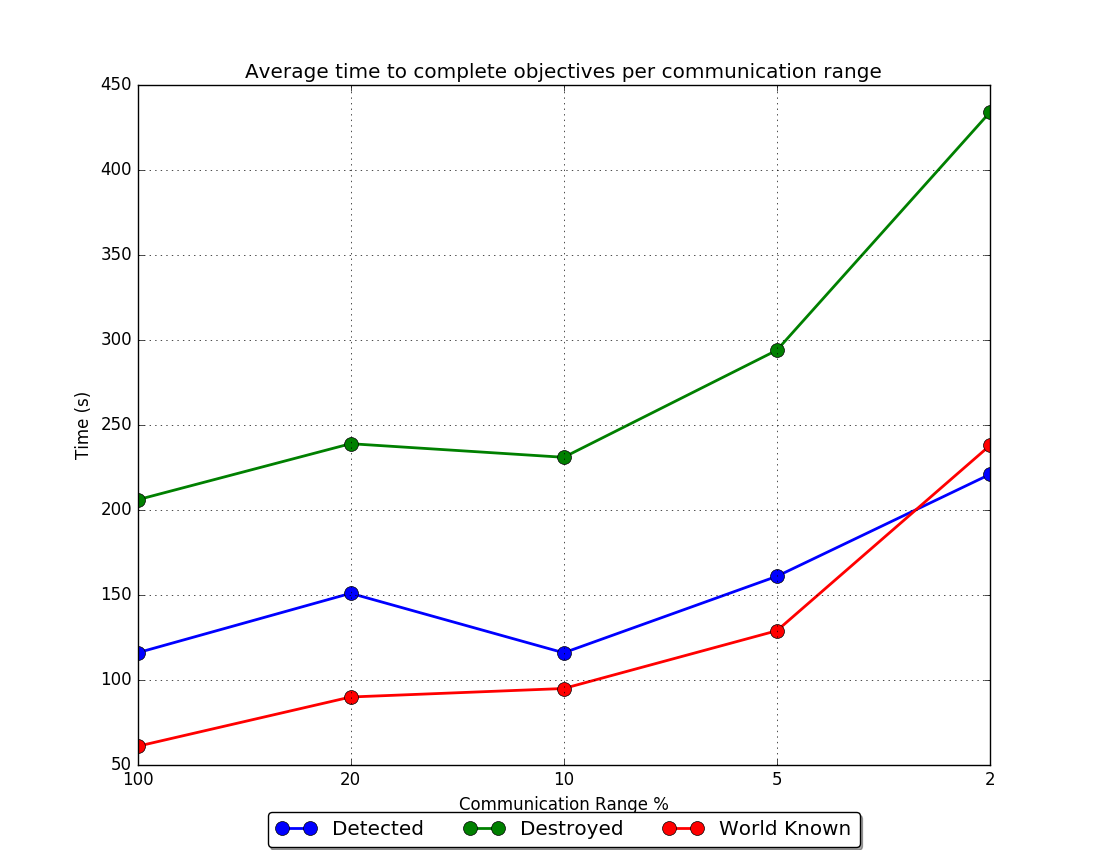
\includegraphics[width=\linewidth,height=3.5in,keepaspectratio=false]{averages.png}
	\caption{Average time to complete objectives per communication range}
	\label{fig:averages}
\end{figure}

\begin{figure}[H]
	\centering
	\includegraphics[width=\linewidth,height=3.5in,keepaspectratio=false]{detected_box.png}
	\caption{Boxplot for time to detect all targets}
	\label{fig:detectBoxPlot}
\end{figure}

\begin{figure}[H]
	\centering
	\includegraphics[width=\linewidth,height=3.5in,keepaspectratio=false]{destroyed_box.png}
	\caption{Boxplot for time to destroy all targets}
	\label{fig:destroyedBoxPlot}
\end{figure}

\begin{figure}[H]
	\centering
	\includegraphics[width=\linewidth,height=3.5in,keepaspectratio=false]{known_box.png}
	\caption{Boxplot for time to know whole world}
	\label{fig:knownBoxPlot}
\end{figure}

\begin{multicols*}{2}

In contrast, the shorter range cases must react quickly once a target is found otherwise there is a strong possibility it will be lost.  This explains why the average time for Detections and World Known are near equal in the $5\%$ case with the average Destroyed time not far behind.  Once a target is seen it is immediately destroyed.

The $2\%$ case shows a similar trend in the time necessary for Detecting and World Known but the Destroyed time is drastically slower.  This is likely because the much shorter range requires the UAVs to frequently give up Monitoring a target since no strike platform is around before the Monitor time out occurs.  In the $2\%$ case the only time a target is struck is when 2 UAVs happen to be near each other when the target is found or a strike UAV happens to be exploring a part of the world it thinks is highly uncertain.  The strike platform will synchronize with the Monitoring UAV and immediately begin the attack process, assuming it has munitions available, otherwise it will have to relay the message to someone else in the swarm.

Within the performance limits and size of the swarm in these simulations we can see that there is no absolute need for every member of a swarm to be able to reach all others in a global fashion.  In practice with standard RF equipment this is actually undesirable because the UAVs will constantly be jamming each other inadvertently.  The standard trade off is finding a suitable transmission range that allows sufficient bandwidth and world coverage between members of the swarm.  Another real world constraint on RF transmissions is the desire to remain undetected.  By limiting our transmission range and power we can limit the range of detectability by enemy RF sensors.  Within the constraints of this simulation we can drop the transmission range down to $10\%$ of the maximum world range with almost no detrimental affects on overall mission performance.  If some performance degradation is acceptable we can further reduce the communication range requirements to $5\%$.  It seems extreme but is also possible to still complete the mission with only a $2\%$ communication range albeit with a much longer mission duration and risk of failure.

\section{Unique Results}
There are a few results where the swarm was unable to complete the mission.  World 3 was a problem for the $100\%$, $10\%$, and $2\%$ cases.  World 3 can be seen in figure~\ref{fig:world3}.  There is a static target located at row 9 column 0.  The best approach angle for striking a static target is $\pm45^{\circ}$.  In this literal edge case that approach angle puts the UAVs on a trajectory outside of the world.  Therefore the UAVs will attempt strikes at very poor angles from the target's backside instead.  The logs show that many shots are taken at this target and miss.  Eventually all of the strike platforms run out of munitions on this target unless they get very lucky.  This result is a limitation of the simulation's random generation nature.  A real world mission analyst would expand the mission area to allow for a better strike angle against this target.  The simulation does not account for accumulating damage.  Every strike is a boolean draw to decide if a target is destroyed or not.  So even though in the simulation dozens of shots were fired at the target it is still considered alive and well.  In the real world dozens of shots would have likely caused significant if not fatal damage to the target even when fired from an undesirable angle.

Communication range case of $5\%$ failed to complete world 4 and case $2\%$ failed to complete world 9.  In both cases a mobile target survived.  The logs show that the Attack platforms and the Monitoring platforms were not in communication range in both cases.  This compounded into multiple problems and possible failure issues.  The strike UAVs, who are the only armed aircraft, have very poor sensors compared to the ISR platforms.  The Attack platforms have a hard time finding and tracking mobile targets with these poor sensors.  Since the Attack and Monitor aircraft were not in communication range the Attack platforms usually had out-dated information and therefore had a tendency to fire where the mobile target was in the past instead of where it is now.  

Another compounding issue in these short communication range cases is that the Monitoring UAVs were strike platforms instead of ISR platforms.  In these cases a strike platform would happen upon a target but no ISR platforms were able to hear about the target announcement.  Therefore the strike platform would perform the Monitoring task and do a poor job of it.  It would follow the mobile target while requesting for a second strike platform to perform the Attack task.  When a strike platform began performing the Attack it would suffer from the same poor sensor issues as the Monitoring platform, leading to many shots at where a target ``was'' instead of where it really ``is.''



\chapter{Conclusions}
foo foo foo

\section{Suggestions for Future Work}
Targets that sense they are under surveillance or attack and evade in response.

False targets/non-combatants.

%\backmatter
\onecolumn
\appendix
\chapter{Appendix}

%------------------------------------------------------------------------------

\section{Dubin's Path} \label{sec:dubin}
The movement of UAVs is constrained to a continuous path with constant speed.

%------------------------------------------------------------------------------

\section{Monitor Sub-states}
\label{sec:monitorSubStates}
\begin{figure}[h]
	\centering
	%\includegraphics[width=\linewidth,height=\textheight]{imagefile}
	\includegraphics[scale=0.6]{uav_monitor_states.png}
	%	\includegraphics{uav_monitor_states.png}
	\caption{Monitor sub-states}
	\label{fig:monitor}
\end{figure}

%------------------------------------------------------------------------------
\section{Attack Activity Diagram}
\label{sec:attackActivity}
\begin{figure}[h]
	\centering
	%\includegraphics[width=\linewidth,height=\textheight]{imagefile}
	\includegraphics[scale=0.6]{uav_activity_attack.png}
	\caption{UAV Attack Activity}
	\label{fig:uavAttackActivity}
\end{figure}

%------------------------------------------------------------------------------

\section{Sample Payload Configurations}
\label{sec:pyldConfigs}
\begin{table}[h]
	\caption{UAV sensor payload configuration}
	\centering
	\rowcolors{1}{lightgray}{white}
	\label{tab:uavSensorMap}
	\begin{tabular}{|p{1cm}|p{1cm}|p{1cm}|}
		\hline
		UAV Type & Sensor Type\\ \hline
		0 & 1 \\
		1 & 0 \\
		\hline
	\end{tabular}
\end{table}

\begin{table}[h]
	\caption{UAV weapon payload configuration}
	\centering
	\rowcolors{1}{lightgray}{white}
	\label{tab:uavWpnMap}
	\begin{tabular}{|p{1cm}|p{1.5cm}|p{2cm}|}
		\hline
		UAV Type & Weapon Type & Initial Quantity\\ \hline
		0 & 0 & 2 \\
		0 & 1 & 2 \\
		1 & 0 & 5 \\
		1 & 1 & 5 \\
		\hline
	\end{tabular}
\end{table}

%------------------------------------------------------------------------------

\section{Algorithms}
\label{sec:algorithms}

\begin{algorithm}
	\caption{UAV Foraging - Selecting a cell to search}
	\label{alg:forage}
	\begin{algorithmic}[1]
		\Function{GenerateForageLocation}{}
			\Require $ 0\le randomWeighting \le 1$
			\Require $ kernelSize \ll min($number world rows, number world columns$)$
			\Require $ \frac{number world rows}{kernelSize} \in Z$
			\Require $ \frac{number world columns}{kernelSize} \in Z$
			\Ensure $ 0 \le x \le $ number world rows
			\Ensure $ 0 \le y \le $ number world columns
			\State $rowsPerKernel\gets $ number world rows $ / kernelSize$
			\State $colsPerKernel\gets $ number world columns $ / kernelSize$		
			\State $x\gets -1$
			\State $y\gets -1$
			\State $maxUncertainty\gets -1$
			\State $maxUncertRow\gets -1$
			\State $maxUncertCol\gets -1$
			
			
			\If{$random() < randomWeighting$}
				\State $ y\gets $ random row
				\State $ x\gets $ random column
			\Else
				\For{$i\gets0$, $i < $number world rows, $i\gets i + rowsPerKernel$}
					\For{$j\gets0$, $j <$ number world columns, $j\gets j + colsPerKernel$}
						\State $kernelUncert\gets computeKernelUncert(i,j, kernelSize)$
						\If{$kernelUncert > maxUncertainty$}
							\State $maxUncertainty\gets kernelUncert$
							\State $maxUncertRow\gets i$
							\State $maxUncertCol\gets j$	
						\EndIf
					\EndFor
				\EndFor
				\State $x\gets randomInteger(rowPerKernel) + maxUncertRow$			
				\State $y\gets randomInteger(colsPerKernel) + maxUncertCol$
			\EndIf \\
			
			\Return x, y
		\EndFunction
	\end{algorithmic}
\end{algorithm}

\begin{algorithm}
	\caption{Cell Belief Merging}
	\label{alg:mergeCell}
	\begin{algorithmic}[1]
		\Function{MergeCells}{$myCells[][], otherCells[][]$}
		\State $numRows\gets $ number of world rows
		\State $numCols\gets $ number of world columns
		\State $alpha\gets $ user defined weighting value in [0,1]
		\For{$i\gets 0, numRows$}
			\For{$j\gets 0, numCols$}
				\If{$otherCells_{ij}.lastUpdateTime > myCells_{ij}.lastUpdateTime$}
					\State $myCells_{ij}.probCellEmpty\gets alpha * otherCells_{ij}.probCellEmpty + (1-alpha) * myCells_{ij}.probCellEmpty$
					\State $myCells_{ij}.lastUpdateTime\gets otherCells_{ij}.lastUpdateTime$
				\EndIf
			\EndFor
		\EndFor
		\EndFunction
	\end{algorithmic}
\end{algorithm}

\begin{algorithm}
	\caption{Target Belief Merging}
	\label{alg:mergeTarget}
	\begin{algorithmic}[1]
		\Function{MergeTargets}{$myTarget, otherTarget$}
		\State $alpha\gets $ user defined weighting value
		\If{$otherTarget.lastUpdateTime > myTarget.lastUpdateTime$}
			\State $myTarget.heading\gets alpha * otherTarget.heading + (1-alpha)*myTarget.heading$
			\State \Call{InterpolateCoordinate}{$myTarget.location, otherTarget.location, alpha$}
			\For{$i\gets 0, $ number of target types}
				\State $myTarget.probTypes[i]\gets alpha * otherTarget.probTypes[i] + (1-alpha)*myTarget.probTypes[i]$
			\EndFor
			\State $myTarget.lastUpdateTime\gets otherTarget.lastUpdateTime$
		\EndIf
		\EndFunction
		\\
		\Function{InterpolateCoordinate}{from, to, percentage}
			\State $deltaNorth\gets to.north - from.north$
			\State $deltaEast\gets to.east - from.east$
			\State $from.north\gets from.north + deltaNorth * percentage$
			\State $from.east\gets from.east + deltaEast * percentage$
		\EndFunction
	\end{algorithmic}
\end{algorithm}

\begin{algorithm}
	\caption{Target Task Status Merging}
	\label{alg:mergeTaskStatus}
	\begin{algorithmic}[1]
		\Function{MergeTargetTaskStatus}{$myTask, otherTask$}
		\State $copyMonitorData\gets false$
		\State $copyAttackData\gets false$
		\\
		\If{$otherTask.monitorState == Complete and myTask.monitorState != otherTask.monitorState$}
			\State $copyMonitorData\gets true$
			\Comment Another UAV completed the task
		\ElsIf{$otherTask.monitorScore > myTask.monitorScore and otherTask.monitorState != Complete and myTask.monitorState != Complete$}
			\State $copyMonitorData\gets true$
			\Comment Everyone is bidding on the task still
		\EndIf
		\\
		\If{$copyMonitorData == true$}
			\State $myTask.monitorID\gets otherTask.monitorID$
			\State $myTask.monitorScore\gets otherTask.monitorScore$
			\State $myTask.monitorState\gets otherTask.monitorState$
			\State $myTask.monitorTimestamp\gets otherTask.monitorTimestamp$									
		\EndIf
		\\
		\If{$otherTask.attackState == Complete and myTask.attackState != otherTask.attackState$}
			\State $copyAttackData\gets true$
			\Comment Another UAV completed the task
		\ElsIf{$otherTask.attackScore > myTask.attackScore and otherTask.attackState != Complete and myTask.attackState != Complete$}
			\State $copyAttackData\gets true$
			\Comment Everyone is bidding on the task still
		\EndIf
		\\
		\If{$copyAttackData == true$}
			\State $myTask.attackID\gets otherTask.attackID$
			\State $myTask.attackScore\gets otherTask.attackScore$
			\State $myTask.attackState\gets otherTask.attackState$
			\State $myTask.attackTimestamp\gets otherTask.attackTimestamp$
			\State $myTask.destroyed\gets otherTask.destroyed$					
		\EndIf

		\EndFunction
	\end{algorithmic}
\end{algorithm}


\begin{algorithm}
	\caption{Task Allocation}
	\label{alg:taskAlloc}
	\begin{algorithmic}[1]
		\State $attackBids \gets $Null Set
		\State $monitorBids \gets $Null Set
		\\
		\If{attacking or monitoring}
			\State Update bid of current task
		\EndIf
		\\
		\For{all targets}
			\State $monitorBids[target] \gets$ compute monitor bid(target)
			\If{Target is pending an attack}
				\State $attackBids[target] \gets$ compute attack bid(target)
			\EndIf
		\EndFor
		\\
		\State $bestMonitorTgt = max(monitorBids)$
		\State $bestAttackTgt = max(attackBids)$
		\\
		\If{$bestAttackTgt$ not null and bid for $bestAttackTgt > $ current belief's task value for target}
			\State Update belief model with bid meta data
			\State Set current task to Attack
		\ElsIf{$bestMonitorTgt$ not null and bid for $bestMonitorTgt > $ current belief's task value for target}
			\State Update belief model with bid meta data		
			\State Set current task to Monitor			
		\Else
			\State Set current task to Search
		\EndIf
		
	\end{algorithmic}
\end{algorithm}
%------------------------------------------------------------------------------

\section{Raw Data}
\begin{table}[H]
	\caption{Time to complete objectives with 100\% Communication range}
	\centering
	\rowcolors{1}{lightgray}{white}
	\label{tab:comm100}
	
	\begin{tabular}{|p{1cm}|p{1.5cm}|p{1.75cm}|p{1.5cm}|p{1.5cm}|}
		\hline
		World & Time all detected (s) & Time all destroyed (s) & Time world known (s) & Time mission complete (s) \\
		\hline
		0&	 86 & 172 & 85 & 172 \\ \hline
		1&	 74 & 159 & 68 & 159 \\ \hline
		2&	111 & 160 & 82 & 160 \\ \hline
		3&	 65 & N/A & 95 & N/A \\ \hline
		4&	191 & 248 & 16 & 248 \\ \hline
		5&	 64 & 175 & 58 & 175 \\ \hline
		6&	205 & 307 & 95 & 307 \\ \hline
		7&	 71 & 130 & 20 & 130 \\ \hline
		8&	118 & 280 & 63 & 280 \\ \hline
		9&	175 & 221 & 29 & 221 \\ \hline
	\end{tabular}
\end{table}



\begin{table}[H]
	\caption{Time to complete objectives with 20\% Communication range}
	\centering
	\rowcolors{1}{lightgray}{white}
	\label{tab:comm20}
	
	\begin{tabular}{|p{1cm}|p{1.5cm}|p{1.75cm}|p{1.5cm}|p{1.5cm}|}
		\hline
		World & Time all detected (s) & Time all destroyed (s) & Time world known (s) & Time mission complete (s) \\
		\hline
		0&122&348&104&348 \\ \hline
		1&66&168&76&168 \\ \hline
		2&176&196&41&196 \\ \hline
		3&61&179&22&179 \\ \hline
		4&144&244&20&244 \\ \hline
		5&117&238&107&238 \\ \hline
		6&238&260&74&260 \\ \hline
		7&166&209&157&209 \\ \hline
		8&261&300&256&300 \\ \hline
		9&156&251&47&251 \\ \hline
	\end{tabular}
\end{table}

\begin{table}[H]
	\caption{Time to complete objectives with 10\% Communication range}
	\centering
	\rowcolors{1}{lightgray}{white}
	\label{tab:comm10}
	
	\begin{tabular}{|p{1cm}|p{1.5cm}|p{1.75cm}|p{1.5cm}|p{1.5cm}|}
		\hline
		World & Time all detected (s) & Time all destroyed (s) & Time world known (s) & Time mission complete (s) \\
		\hline
		0&119&305&117&305 \\ \hline
		1&102&378&144&378 \\ \hline
		2&217&294&104&294 \\ \hline
		3&55&N/A&41&N/A\\ \hline
		4&74&174&19&174 \\ \hline
		5&198&244&184&244 \\ \hline
		6&119&170&91&170 \\ \hline
		7&109&222&53&222 \\ \hline
		8&123&165&124&165 \\ \hline
		9&44&125&69&125 \\ \hline

	\end{tabular}
\end{table}


\begin{table}[H]
	\caption{Time to complete objectives with 5\% Communication range}
	\centering
	\rowcolors{1}{lightgray}{white}
	\label{tab:comm5}
	
	\begin{tabular}{|p{1cm}|p{1.5cm}|p{1.75cm}|p{1.5cm}|p{1.5cm}|}
		\hline
		World & Time all detected (s) & Time all destroyed (s) & Time world known (s) & Time mission complete (s) \\
		\hline
		0&238&279&242&279 \\ \hline
		1&112&237&123&237 \\ \hline
		2&164&199&85&199 \\ \hline
		3&55&351&65&351 \\ \hline
		4&76& N/A &66& N/A\\ \hline
		5&171&263&136&263 \\ \hline
		6&394&424&161&424 \\ \hline
		7&172&440&142&440 \\ \hline
		8&133&244&156&244 \\ \hline
		9&100&210&115&210 \\ \hline
	\end{tabular}
\end{table}


\begin{table}[H]
	\caption{Time to complete objectives with 2\% Communication range}
	\centering
	\rowcolors{1}{lightgray}{white}
	\label{tab:comm2}
	
	\begin{tabular}{|p{1cm}|p{1.5cm}|p{1.75cm}|p{1.5cm}|p{1.5cm}|}
		\hline
		World & Time all detected (s) & Time all destroyed (s) & Time world known (s) & Time mission complete (s) \\
		\hline
		0&380&554&339&554 \\ \hline
		1&167&498&468&498 \\ \hline
		2&288&596&233&596 \\ \hline
		3&50& N/A &164& N/A\\ \hline
		4&269&337&93&337 \\ \hline
		5&261&299&166&299 \\ \hline
		6&199&395&332&395 \\ \hline
		7&257&468&183&468 \\ \hline
		8&234&323&293&323 \\ \hline
		9&103& N/A &110& N/A\\ \hline
	\end{tabular}
\end{table}

\section{Data type models}
TBD
\todo{Create UML data type/structure models here.}

%This gets the Bibliography to appear in the table of contents by generating the header manually
\chapter{Bibliography}
\printbibliography[heading=none]


%Notes to the author
\listoftodos

%\chapter{DELETE ME. Unused Proposal text}

As in \cite{jin} three styles of task assignment algorithms will be compared.  The base line tasking algorithm will allocate tasks in real-time as they appear.   A predictive algorithm will attempt to predict a chain of tasks before they occur and move members of the swarm into position ready to perform a task before it is generated.  This could occur when a target is first seen but not yet confirmed.   As a sensing aircraft confirms the target identity and orientation an attack aircraft could move into position and be prepared to strike after the confirmation task is complete.  The predictive algorithm causes a trade-off between search (exploration) and response (exploitation).  A third algorithm is a hybrid of the baseline and predictive algorithms that will try to merge the best of both algorithms.  It will default to exploring as in the baseline until certain criteria about the world are known and then it will switch to a predictive behavior until the criteria are no longer satisfied.

Payloads are one of the most costly elements on aircraft and the more functionality a payload has the more it typically costs.  As noted earlier, Jin’s model assumed only forward facing sensors.  One case study for this project will be to compare the performance of the three algorithms using static forward facing sensors against the performance of using gimballed sensors.  Intuitively gimballed sensors should provide more flexibility in the trajectories of aircraft allowing them to reach new tasks faster.  This case study will confirm whether this is true or not and if it is true will determine if gimballed sensors have enough of a benefit to warrant the additional cost, power requirements, and weight added to an aircraft.  

Additionally the performance comparison between gimballed and fixed sensors will be done over a wide range of swarm sizes.  It’s likely that there is a critical point where the size of a swarm is large enough that fixed sensors are equivalent in performance to fewer gimballed sensors.  In essence this will look for the point where the performance of many cheaper UAVs is comparable to fewer more expensive UAVs.

The second case study will explore the effects upon performance due to varying intra-swarm communication ranges.  The ranges will vary from no intra-swarm communication to a global communication range.  The control parameters for this study are the average density of the swarm per unit area and the range of communication.  Plotting the average density of the swarm, the communication range of the members, and the average total mission times will produce a three dimensional manifold.  The equation describing the shape of this manifold can be used to predict the number of UAVs needed to minimize total mission time given the communication range limits of the UAVs.

The data produced by both case studies can also be used for another purpose.  Each measures how the size of the swarm affects mission efficiency.  Based on this data we should be able to draw a conclusion on whether it’s more efficient to utilize a UAV’s size, weight, and power budget on better communication systems or better sensors.

The innovation in this project comes from creating a system that can readily be applied to real world situations.  The goal is not to create a better Pursuit-Evasion or Weapon Target Assignment solution.  The goal is to create a system that can merge the two problems, regardless of how those subdomains are solved, within a limited or disrupted communication environment.  This will advance the scientific domain of operations research for multi-agent coordinated mission and resource management.

Coordinating the efforts of multiple aircraft in a small airspace is difficult and dangerous.  Add in limited or disrupted communications and the amount of risk involved dramatically increases.  This mission management work requires many people to operate together and all the supporting equipment that goes with it. The algorithm generated by this research can automate this coordination process.  Automation will allow much faster and much more accurate modeling of the region compared to a group of people.  The algorithm can serve as air traffic controllers, pilots, and mission controllers simultaneously.  This means aircraft can fly closer together allowing more aircraft to be utilized simultaneously in a small area increasing the probability of mission success in a timely fashion.

The results of this work should make it possible for a single person to direct a swarm of UAVs.   This has applicability to military, disaster response, search and rescue, border protection, aerial firefighting, and precision agriculture scenarios.

The two case studies focus on how the size of the swarm affects mission performance.  The results will help future swarm creators determine how best to design a swarm.  Should fewer more advanced aircraft be used or should many simple aircraft be used?  The data from the case studies can help answer these questions.   Furthermore the equations derived from the communication manifold case can be used to estimate how many UAVs are needed in a swarm to complete the objectives within a timely manner given the characteristics of the swarm’s aircraft.  It can also be used as a predictive model for determining the probability of a success of a mission after losing members of a swarm.  The swarm operators should know the available flight time or operational time left in the swarm before the aircraft run out of fuel or power.  Comparing this time against the predicted time to complete a mission could provide a rough estimate on the probability of mission success.
\end{document}
